\documentclass[journal]{vgtc}                % final (journal style)
%\documentclass[review,journal]{vgtc}         % review (journal style)
%\documentclass[widereview]{vgtc}             % wide-spaced review
%\documentclass[preprint,journal]{vgtc}       % preprint (journal style)
%\documentclass[electronic,journal]{vgtc}     % electronic version, journal

%% Uncomment one of the lines above depending on where your paper is
%% in the conference process. ``review'' and ``widereview'' are for review
%% submission, ``preprint'' is for pre-publication, and the final version
%% doesn't use a specific qualifier. Further, ``electronic'' includes
%% hyperreferences for more convenient online viewing.

%% Please use one of the ``review'' options in combination with the
%% assigned online id (see below) ONLY if your paper uses a double blind
%% review process. Some conferences, like IEEE Vis and InfoVis, have NOT
%% in the past.

%% Please note that the use of figures other than the optional teaser is not permitted on the first page
%% of the journal version.  Figures should begin on the second page and be
%% in CMYK or Grey scale format, otherwise, colour shifting may occur
%% during the printing process.  Papers submitted with figures other than the optional teaser on the
%% first page will be refused.

%% These three lines bring in essential packages: ``mathptmx'' for Type 1
%% typefaces, ``graphicx'' for inclusion of EPS figures. and ``times''
%% for proper handling of the times font family.
\usepackage{amssymb}
\usepackage{mathptmx}
\usepackage{graphicx}
\usepackage{times}

%% We encourage the use of mathptmx for consistent usage of times font
%% throughout the proceedings. However, if you encounter conflicts
%% with other math-related packages, you may want to disable it.

%% This turns references into clickable hyperlinks.
\usepackage[bookmarks,backref=true,linkcolor=black]{hyperref} %,colorlinks
\hypersetup{
  pdfauthor = {},
  pdftitle = {},
  pdfsubject = {},
  pdfkeywords = {},
  colorlinks=true,
  linkcolor= black,
  citecolor= black,
  pageanchor=true,
  urlcolor = black,
  plainpages = false,
  linktocpage
}

%% If you are submitting a paper to a conference for review with a double
%% blind reviewing process, please replace the value ``0'' below with your
%% OnlineID. Otherwise, you may safely leave it at ``0''.
\onlineid{0}

%% declare the category of your paper, only shown in review mode
\vgtccategory{Research}

%% allow for this line if you want the electronic option to work properly
\vgtcinsertpkg

%% In preprint mode you may define your own headline.
%\preprinttext{To appear in IEEE Transactions on Visualization and Computer Graphics.}

%% Paper title.

\title{MetaTracts - A Method for Robust Extraction and Visualization of Carbon Fiber Bundles in Fiber Reinforced Composites}

%% This is how authors are specified in the journal style

%% indicate IEEE Member or Student Member in form indicated below

\author{Arindam Bhattacharya\thanks{e-mail: arindamb86@gmail.com}\\ %
	\scriptsize The Ohio State University %
	\and Christoph Heinzl\thanks{e-mail:christoph.heinzl@fh-wels.at}\\ %
	\scriptsize University of Applied Sciences - Upper Austria%
	\and Artem Amirkhanov\thanks{e-mail:artem.amirkhanov@fh-wels.at}\\ %
	\scriptsize University of Applied Sciences - Upper Austria%
	\and Johann Kastner\thanks{e-mail:johann.kastner@fh-wels.at}\\ %
	\scriptsize University of Applied Sciences - Upper Austria%
	\and Rephael Wenger\thanks{e-mail:wenger@cse.ohio-state.edu}\\ %
	\scriptsize The Ohio State University
}

%\author{Arindam Bhattacharya, , and Martha Stewart}
%\authorfooter{
%% insert punctuation at end of each item
%\item
% Roy G. Biv is with Starbucks Research. E-mail: roy.g.biv@aol.com.
%\item
% Ed Grimley is with Grimley Widgets, Inc.. E-mail: ed.grimley@aol.com.
%\item
% Martha Stewart is with Martha Stewart Enterprises at Microsoft
% Research. E-mail: martha.stewart@marthastewart.com.
%}

%other entries to be set up for journal
\shortauthortitle{Biv \MakeLowercase{\textit{et al.}}: Global Illumination for Fun and Profit}
%\shortauthortitle{Firstauthor \MakeLowercase{\textit{et al.}}: Paper Title}

%% Abstract section.
\abstract{Duis autem vel eum iriure dolor in hendrerit in vulputate
velit esse molestie consequat, vel illum dolore eu feugiat nulla
facilisis at vero eros et accumsan et iusto odio dignissim qui blandit
praesent luptatum zzril delenit augue duis dolore te feugait nulla
facilisi. Lorem ipsum dolor sit amet, consectetuer adipiscing elit,
sed diam nonummy nibh euismod tincidunt ut laoreet dolore magna
aliquam erat volutpat. Ut wisi enim ad minim veniam, quis nostrud exerci tation ullamcorper
suscipit lobortis nisl ut aliquip ex ea commodo consequat. Duis autem
vel eum iriure dolor in hendrerit in vulputate velit esse molestie
consequat, vel illum dolore eu feugiat nulla facilisis at vero eros et
accumsan et iusto odio dignissim qui blandit praesent luptatum zzril
delenit augue duis dolore te feugait nulla facilisi.
} % end of abstract

%% Keywords that describe your work. Will show as 'Index Terms' in journal
%% please capitalize first letter and insert punctuation after last keyword
\keywords{Radiosity, global illumination, constant time}

%% ACM Computing Classification System (CCS). 
%% See <http://www.acm.org/class/1998/> for details.
%% The ``\CCScat'' command takes four arguments.

\CCScatlist{ % not used in journal version
 \CCScat{K.6.1}{Management of Computing and Information Systems}%
{Project and People Management}{Life Cycle};
 \CCScat{K.7.m}{The Computing Profession}{Miscellaneous}{Ethics}
}

%% Uncomment below to include a teaser figure.
%   \teaser{
%   \centering
%   \includegraphics[width=16cm]{CypressView}
%   \caption{In the Clouds: Vancouver from Cypress Mountain.}
%  }

%% Uncomment below to disable the manuscript note
%\renewcommand{\manuscriptnotetxt}{}

%% Copyright space is enabled by default as required by guidelines.
%% It is disabled by the 'review' option or via the following command:
% \nocopyrightspace

%%%%%%%%%%%%%%%%%%%%%%%%%%%%%%%%%%%%%%%%%%%%%%%%%%%%%%%%%%%%%%%%
%%%%%%%%%%%%%%%%%%%%%% START OF THE PAPER %%%%%%%%%%%%%%%%%%%%%%
%%%%%%%%%%%%%%%%%%%%%%%%%%%%%%%%%%%%%%%%%%%%%%%%%%%%%%%%%%%%%%%%%

%% Commands
\newcommand{\mt}{MetaTracts }

\begin{document}

%% The ``\maketitle'' command must be the first command after the
%% ``\begin{document}'' command. It prepares and prints the title block.

%% the only exception to this rule is the \firstsection command
%%\firstsection{Introduction And Motivation}


\maketitle
\section{Introduction And Motivation}\label{sec:intro}
Modern industry is increasingly demanding function orientation, integration, and efficiency of novel materials and components. The material of choice for a growing number of applications is carbon fiber reinforced polymer (CFRP), which allows an integration of these continuously rising demands and increasingly replaces conventional materials such as aluminum or steel.
 CFRP materials have desirable characteristics such as high specific stiffness, high specific strength and high corrosion resistance. Moreover, CFRP materials show these characteristics at considerably lower weight. At the same time, highly complex and integrated components, which were previously impossible to manufacture may be produced from CFRPs. Primary structures and highly loaded components in aeronautics are one example. Typically, carbon fiber reinforced polymer components and more specifically CFRP laminates with endless carbon fibers as addressed in this work consist of two main components:
a matrix, which acts as a bonding component, and the reinforcements, which allow for achieving the desired characteristics. Various production processes are used to manufacture CFRP laminates. Most of these processes start with the reinforcement component, weaving individual carbon fiber bundles (yarn) into sheets of carbon fiber cloth in a predefined pattern. These sheets of woven carbon fiber cloth are also referred to as fabric and form the geometrical structure of the final CFRP materials. Depending on the requirements of the final component, fabrics may be stacked in multiple layers in similar or different orientation. Both the  alignment of fabrics and the weaving pattern of the individual carbon fiber bundles strongly influence the properties of the CFRP laminate. Resins are then integrated in the material system to fill the gaps in the fabric forming the matrix component. The main function of the matrix is to act as a bonding between the individual carbon fiber bundles. After curing, the production process of the CFRP laminate is finished.

The increasing share of CFRPs as well as the complexity of both material system and final component has generated a strong demand towards non-destructive testing (NDT) techniques for quality control~\cite{Red2012}. Ultrasonic testing (UT) is the most commonly used method for this purpose. While UT provides a quick and cost-efficient overview of the material, it also lacks resolution and may generate arbitrary results, e.g., due to the geometry of the component. Industrial 3D X-ray computed tomography (XCT, also referred to as 3DXCT or cone beam XCT) is increasingly applied for non-destructive testing of fiber reinforced polymers~\cite{Kastner2012}. In contrast to UT, XCT generates a highly detailed 3D volumetric representation of the scanned specimen. In cone beam XCT geometry the specimen is placed on a rotary table between X-ray source and detector. The X-rays passing through the specimen get attenuated by the materials present. By transferring the X-rays in a scintillator layer into visible light, the detector records the corresponding 2D attenuation image (penetration image). The specimen is rotated, recording at each angular step a 2D attenuation image to generate the full series of attenuation images of a $360^\circ$ rotation required for a complete reconstruction of the data volume ~\cite{heinzl-2008-thesis}. 
While cone beam XCT can reach voxel sizes below 500 $nm$ generating high resolution volume data for comprehensive and detailed analyses, unfortunately there is still a trade-off between viewport and image resolution. The magnification reached within an XCT scan is determined by the distances between source and specimen as well as source and detector. The magnification therefore directly influences both resolution and viewport: while higher resolutions decrease the viewport but show more details, lower resolutions allow for larger viewports and thus larger portions of the specimen.

In this work, we focus on datasets with larger viewports but
lower resolutions where the individual carbon fibers (filaments) are indiscernible or barely visible. Our domain experts are mainly interested in visualizing the geometric structures in the weaving pattern of fiber bundles in endless carbon fiber reinforced composites instead of high resolution studies of individual fibers.
%of short fiber reinforced composites as presented by Weissenbock2014 et al.~\cite{Weissenbock2014}.
Figure~\ref{fig:data-char} depicts our targeted dataset type. It shows the recurring fiber bundle pattern in the final CFRP laminate, the \textit{unit cell}.
Our work is motivated from the recent progress in two interrelated fields: Firstly, CFRP components have gained wide application in industry because of its superior material and physical properties in comparison to conventional materials~\cite{Karpat2012}. Secondly, recent developments of industrial 3D X-ray computed tomography (XCT) with regard to larger detectors, larger field of views, and better resolutions opened XCT for this new application area of non destructive testing for fiber reinforced components~\cite{Schilling2005}. 

While fiber bundles are now understood as highly important in determining component properties, the tools for visualizing the internal structure have not developed at the same pace.
To the best of our knowledge, there is no current work that can resolve simple queries such as:
\begin{itemize}[noitemsep]
	\item{ How to extract and visualize the geometric structure of a particular fiber bundle?}
	\item{ How to visualize the interaction between a particular pair of fiber bundles (weaving/braiding) or a unit cell?}
	\item{ Which fiber bundles show a particular orientation? }
	\item{ Which fiber bundles are of the same type of yarn? I.e. which bundles show similar sizes or diameters, which is the largest or smallest fiber bundle ?}
\end{itemize}

We demarcate the above queries into two parts: \textit{geometric structure} and \textit{spatial context}. Geometric structure refers to the shape, size, and orientation of a fiber bundle or a group of them. Spatial context refers to how two or more bundles interact with each other.It provides answers to questions such as: Are these bundles in contact at a particular position in the data? What are the relative orientations of the contacting bundles? 
Providing answers to the above queries from the volume renderings of XCT datasets or from visual inspection of particular 2D slices is non-trivial, even for experts. We present and evaluate a method which uses visualization techniques to gain insight into our data.
We interpret and advance techniques from diffusion tensor imaging to extract and visualize geometric structures from 3D X-ray computed tomography data of the woven carbon fiber reinforced composites. The main goal of this work is to expand the state of the art in non-destructive testing through visualization of composite structures in \textit{complete unit cells} of woven fabrics.
\begin{figure}[htb]
	\centering
	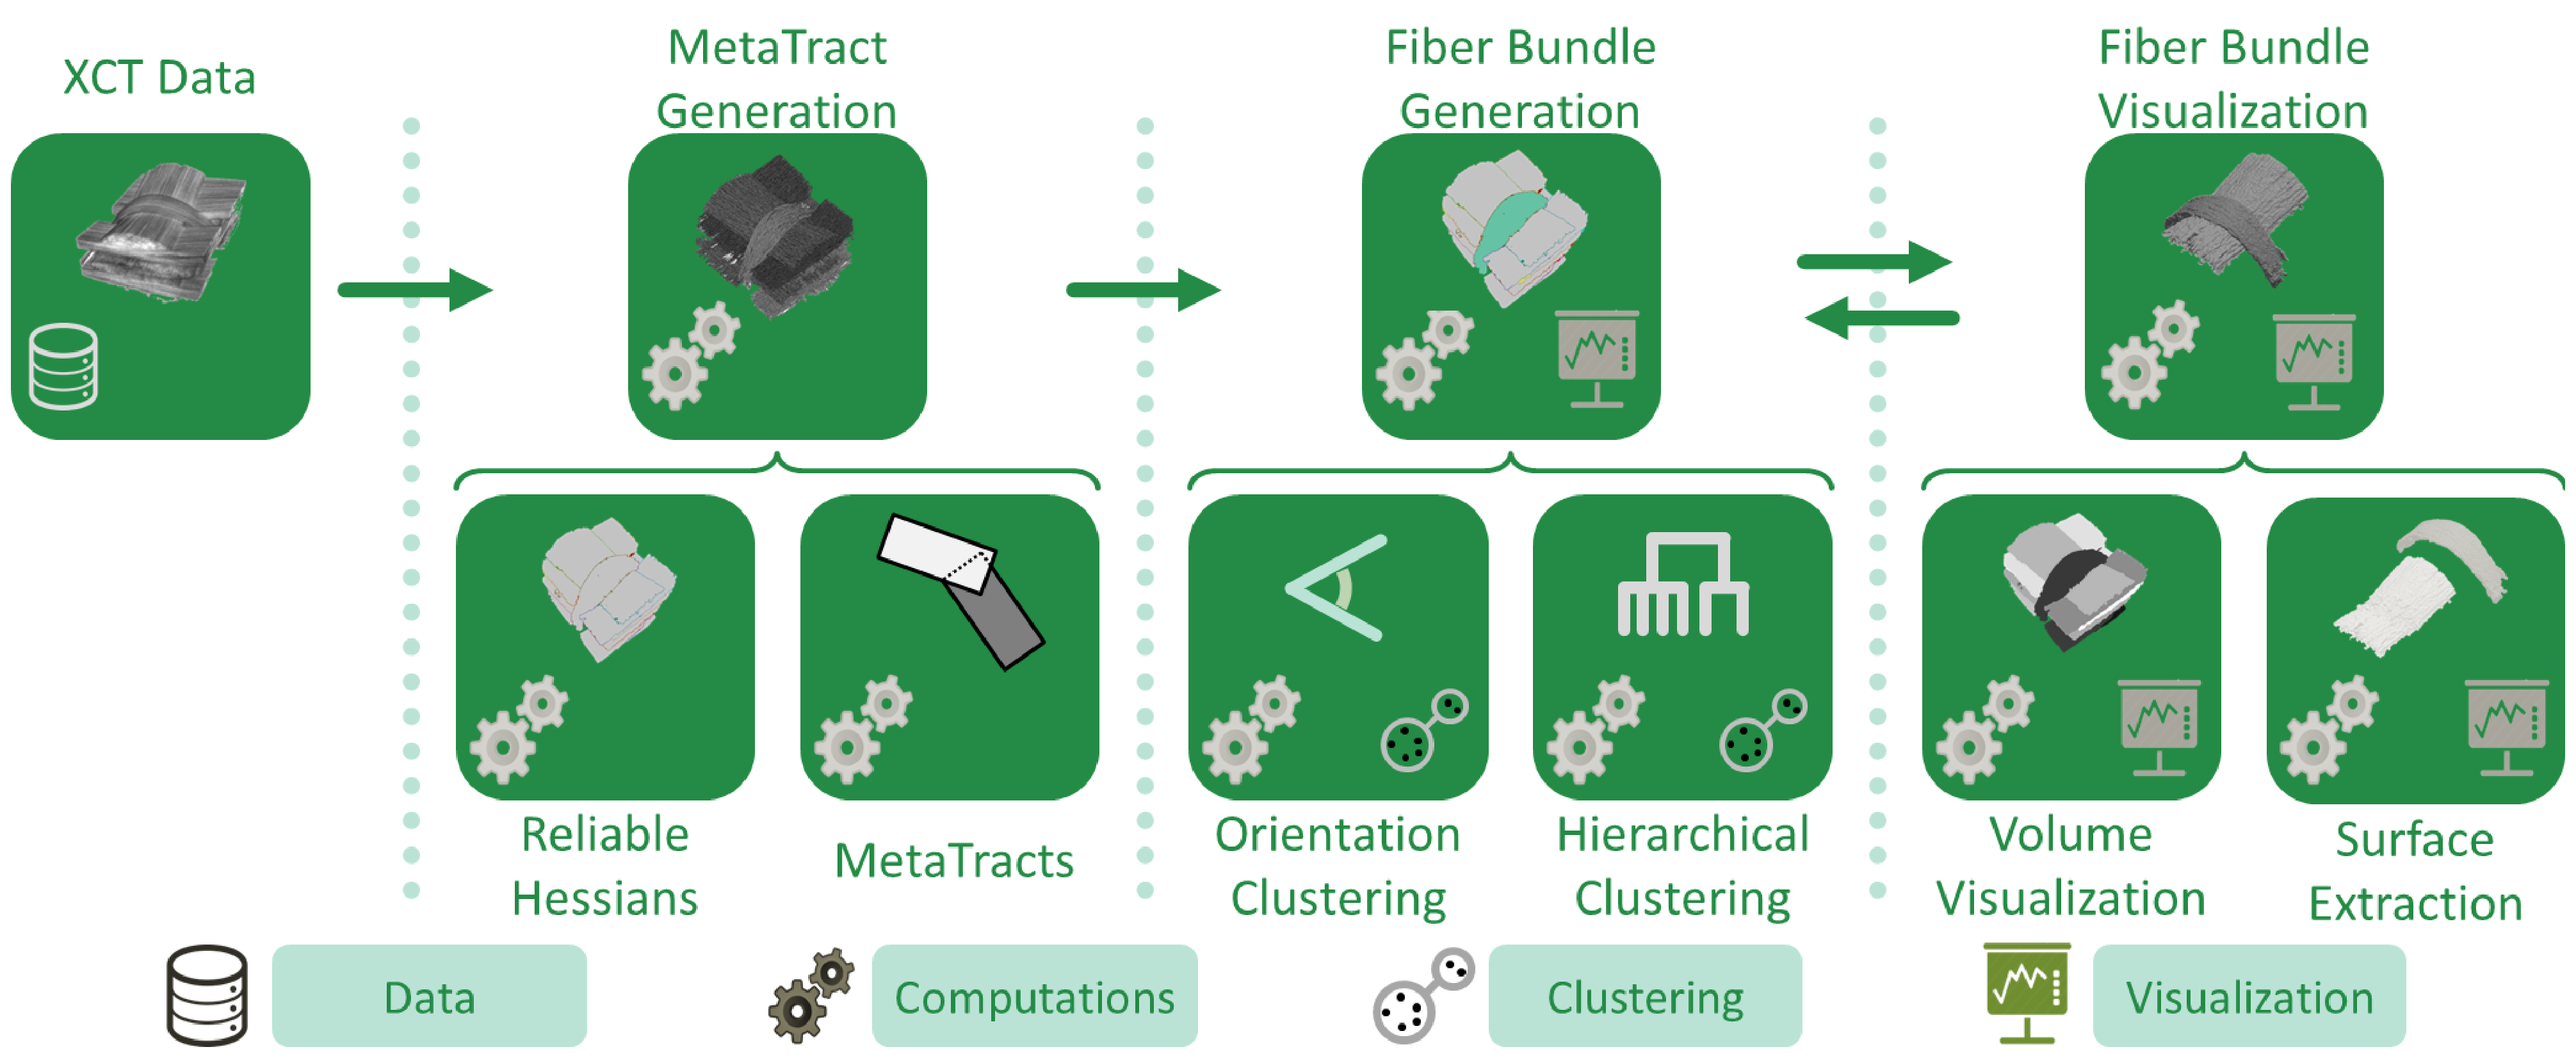
\includegraphics[width=\linewidth]{images/workflow.eps}
	\caption{Flow chart of the MetaTracts approach for fiber bundle extraction}
	\label{fig:flowchart}
\end{figure}
Figure~\ref{fig:flowchart} shows an over view of our approach.
Starting from XCT data, we first generate MetaTracts (see Sec.~\ref{sec:ext_mt}). Then we cluster the MetaTracts to generate and visualize fiber bundles (see Sec.~\ref{subsec:fiber-bundles}). We discuss the visualizations we created for our domain experts in Sec.~\ref{sec:vis}. Sec.~\ref{sec:results} describes our experimental results, Sec.~\ref{sec:param_choices} presents our parameter choices and  Sec.~\ref{sec:user_eval} summarizes the user evaluation of our method.

\section{Related Work}
Diffusion Magnetic Resonance Imagining (dMRI, also referred to as Diffusion Tensor Imaging (DTI)) is a magnetic resonance imaging technique which provides three-dimensional information about the structures in cerebral white matter based on diffusion of water molecules. DTI has gained popularity in medical diagnosis within recent years; its main clinical application is found in the study and treatment of neurological disorders. DTI may reveal abnormalities in white matter fiber structure and is used for visualizing the organization of fibers in the human brain and brain connectivity.
A variety of algorithms have been proposed for generating fiber-tract trajectories. In general, these reconstructions of fiber trajectories are clustered into bundles which are expected to be related anatomically or spatially. 
We broadly divide the related work on DTI into two parts of immediate relevance to our proposed solution: fiber tracking and fiber clustering. We next review methods for analyzing the second order local structure and the current state of the art in the visual analysis of fiber reinforced composites.
\subsection {Fiber Tracking in Diffusion Tensor Imaging}
\label{subsec:fiberEx} 
A basic assumption in DTI analysis is that the principal eigenvector of the diffusion tensor is parallel to the underlying dominant fiber direction in each image voxel~\cite{Basser2002, Mori1999, Mori2002}. The principal diffusion direction at each discrete location is interpolated to form a continuous velocity field. Continuous tracts are generated by propagating virtual particles along the principal diffusion directions until they reach some termination criterion. 
This is usually done by solving a Runge-Kutta integration (typically second or fourth order).
Because decisions are made locally, these methods perform poorly in noisy regions and often generate small fibers. Basser et al.~\cite{Basser2002,Basser2000} proposed that white matter tracts could be represented as 3D curves in space. They showed that numerical methods could be used to follow fibers and fiber bundles and to generate tracts in human brain data. 
Mori et al.~\cite{Mori1999,Mori2002} divided reconstruction techniques into line-propagation or energy minimization techniques. In line propagation approaches, trajectories are computed based on local neighborhoods and in energy minimization approaches the most favorable trajectory connecting two given endpoints is selected. 


\subsection {Fiber Clustering in Diffusion Tensor Imaging}
\label {subsec:fiberClus}
In DTI, similarity measures such as proximity between fibers are used to group fiber tracts into bundles. Extensive research has been done on automatic DTI fiber clustering methods \cite{Brun2004,Brun2003,Corouge2004,westinMEDIA02,Zhang2008}. These approaches build on the assumption that proximity measures that compare DTI fiber trajectories can also represent anatomical relationships.
Clustering requires choosing a suitable proximity measure and a method for grouping ``close" fibers.

Pairwise proximity measures include endpoint distances~\cite{Brun2003} and mean of the closest distances between points on two fibers~\cite{Corouge2004}. Zhang et al.~\cite{Zhang2008} introduced a thresholded version of the closest distances mean, so that fibers which are close for certain distance and then diverge, are clustered separately. Brun et al.~\cite{Brun2004} use normalized cuts along with a pairwise distances measure computed using a 9D fiber shape descriptors. 

The choice of the clustering algorithm can be broadly divided into those approaches using hierarchical clustering~\cite{Moberts2005, Zhang2008} and those using spectral clustering~\cite{Brun2004,jonasson2005, ODonnell2007}.
Brun et al.~\cite{Brun2003} described how a spectral non-linear dimensionality reduction technique, Laplacian eigenmaps (Belkin and Niyogi~\cite{Belkin01}), can be applied to the problem of organizing fiber tracts data. The key notion of the Laplacian eigenmaps algorithm is to represent the underlying data as a graph. Each node represents a data point and the edges connect neighboring data points. An eigenvalue problem is solved to represent the data in a lower dimensional space while preserving the local graph structure. In the case of fiber bundles, the individual points are fiber tracts. In the ideal case fiber tracts belonging to the same bundle must remain ``close" to each other in the lower dimensional space. Westin et al.~\cite{westinMEDIA02} also used spectral clustering on a Hausdorff distance measure defined as the maximum of point wise minimum distances between two fibers. Jonasson et al.~\cite{jonasson2005} ran k-means clustering on the eigenvectors of the affinity matrix defined as the co-occurrence of fibers in the data.
Additionally, the agglomerative hierarchical clustering method~\cite{DudaHartStork01} has gained popularity for proximity based fiber segregation (Zhang et al.~\cite{Zhang2008}, Corouge et al.~\cite{Corouge2004}). 
An agglomerative hierarchical clustering method starts with each data point/fiber in an individual cluster. At each stage of the algorithm the two most similar clusters are merged based on some criterion. The two basic cluster similarity measures are single-link and complete-link. With the single link, the distance between the clusters is the distance between the closest pair of items. 
Moberts et al.~\cite{Moberts2005} implemented several distance measures in their evaluation of fiber clustering and concluded that clustering methods are generally accurate in capturing fiber bundles. 
 
There are a number of difficulties in hierarchical clustering. First, computing all pairs' distances for tracts to generate the distance matrix is time consuming~\cite{Garyfallidis2012}. Second, a ``correct'' distance measure to compare tracts must be chosen. Third, hierarchical clustering is best suited for similar length fibers.
Spectral methods are also hindered by long matrix computations.


\subsection{Second order local structure}
Unlike DTI, we do not have diffusion tensor data. Instead, we have a scalar volume with tubular structures embedded in them. Analyzing curvilinear structures in volumetric images has been utilized for a variety of purposes including center line extraction~\cite{Bouix2005} and vascular image enhancement as proposed by Frangi et al.~\cite{Frangi1998} and Sato et al.~\cite{Sato1997}. Frangi et al.~\cite{Frangi1998} introduced a method based on studying the eigenvalues of the Hessian matrix specifically for the purposes of developing vessel enhancement filters.

\subsection {Visual Analysis and Modeling of Fiber Reinforced Composites}
The approaches presented in visualization and analysis of composites mainly focuses on individual objects such as fiber extraction from high resolution data where the individual fibers are clearly discernible. Fritz et al.~\cite{Fritz2009} proposed interactive workflows for non destructive testing practitioners to explore and quantify steel fibers in reinforced sprayed concrete. %This approach allows analyzing fiber orientations based on direction transfer functions. 
Salaberger et al.~\cite{Salaberger2011} introduced a pipeline to extract and characterize individual fibers of fiber reinforced composites. They encode the extracted fibers as color-coded line segments in 3D and visually identifying fibers with similar orientations.
Recently, Weissenb{\"o}ck et al.~\cite{Weissenbock2014} presented a system for interactive exploration and analysis of fibers in fiber reinforced polymers.
They use the visualization paradigms of a scatter plot matrix and parallel coordinates to select fibers according to their characteristics. The defined fiber classes can be managed in a list and are displayed with a 3D renderer.  
Lomov et al.~\cite{Lomov2010} discusses the problems and current available solutions in geometric modeling of three dimensional composites.
Modeling of the composites, first starts with establishing the topology of the structure, which translates to answering if a particular bundle is in contact with another at a particular position? The second step builds the geometry of the model, answering queries relating to placement of bundles in space, their orientations and dimensions. 
\begin{figure}[htb]
\centering
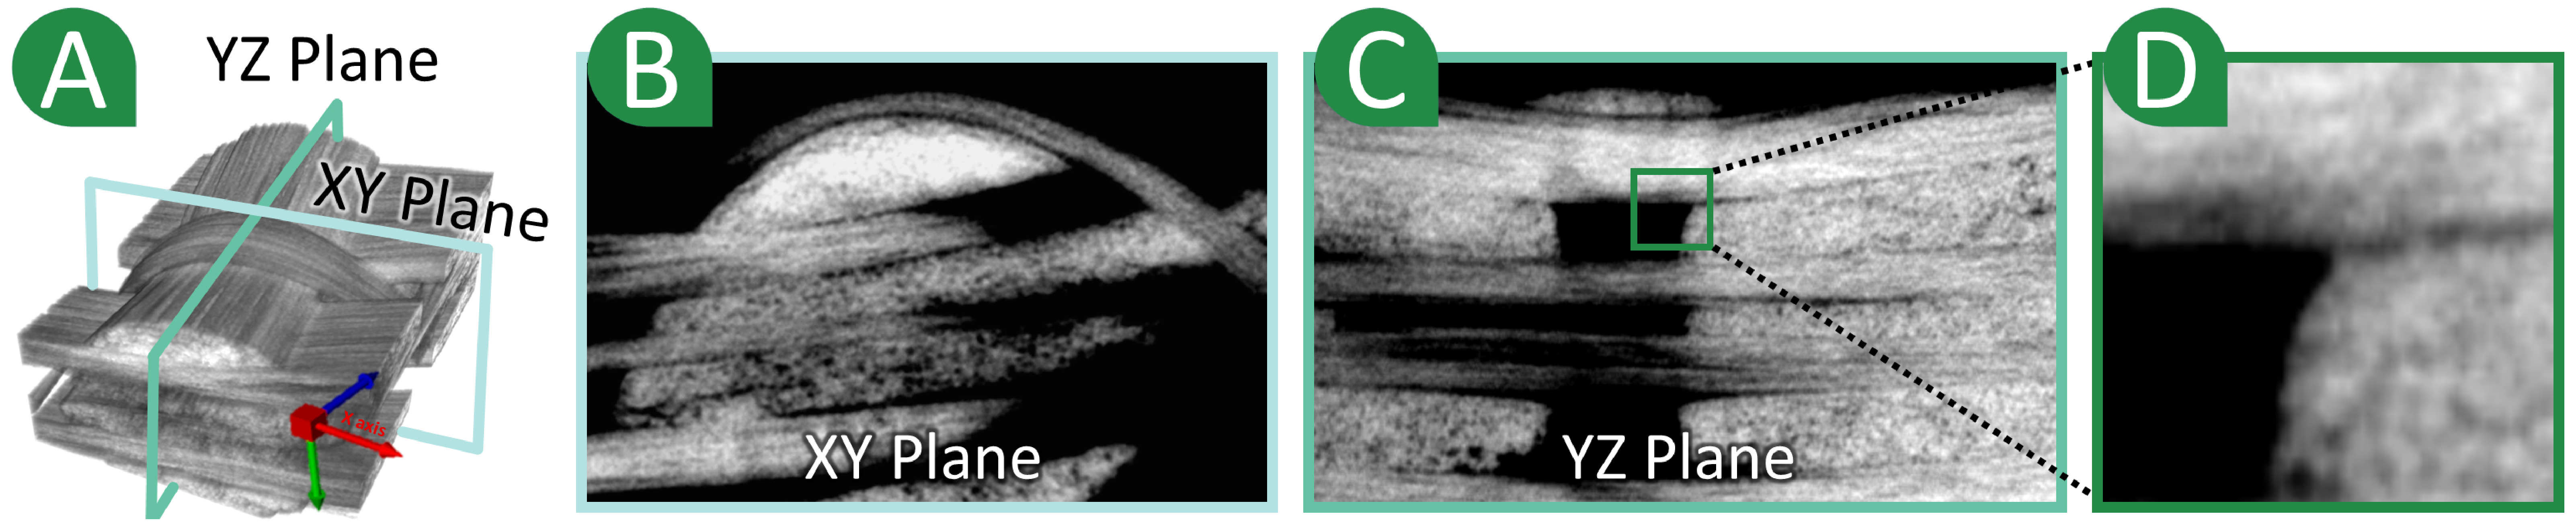
\includegraphics[width=\linewidth]{images/data-char.eps}
\caption
{
Data characteristics: (a) Rendering of dataset D1. (b, c) 2D slices along Z- and X-axis. (d) Zoom in of the green region marked in (c). Multiple fiber bundles cross and are indistinguishable by visual inspection alone. 
}
\label{fig:data-char}
\end{figure}

\section {Data Characteristic and Assumptions}
\label{sec:char_data}
Figure~\ref{fig:data-char} shows dataset D1 with woven fiber bundles. The size of D1 is 450$\times$300$\times$500 voxels with isotropic resolution of 2 $\mu m$ and 8 bit unsigned integer scalars. Figure~\ref{fig:data-char} clearly shows the recurring fiber bundle weaving pattern of the composite unit cell used for manufacturing fiber composites. Figure~\ref{fig:data-char}\brac{a} shows a volume rendering of the dataset. Figure~\ref{fig:data-char}\brac{b} and ~\ref{fig:data-char}\brac{c} show 2D slices along the $X$- and the $Z$-axis respectively. Figure~\ref{fig:data-char}d zooms into the green region of interest. 
Figure~\ref{fig:data-char}\brac{d} contains two bundles going in opposite directions, the low resolution of D1 renders the individual carbon fibers in a fiber bundle hard to resolve. Also the separation between two fiber bundles is barely visible. The fiber bundles may differ in terms of the amount of fibers in the bundle. Figure~\ref{fig:data-char}\brac{a} shows the large variation in cross section sizes among the bundles.
Depending on the weaving pattern, the fiber bundles cross each other in different orientations. The number of orientations is defined by the weaving pattern and typically consists of two main orientations. The weaving pattern may cause individual bundles to be curved. In consequence, individual fibers may be adjacent in Euclidean distance but belong to different bundles. 
We make the following \textit{assumptions} on our data:

\begin{itemize}[noitemsep]
\item The structure embedded in the data contains fiber bundles of indiscernible fibers.
\item Local orientation: each point in a fiber bundle has a local orientation parallel to the corresponding area in the fiber bundle.
\item Local orientation may gradually change within the fiber bundle.
\item Local orientation may be noisy and not reliable.
\item Connectivity: moving along the direction of a non-noisy local orientation in small increments, we will reach another neighborhood with similar local orientation.
\item Fiber bundles going in different directions only interact near the surface of contact.
\end{itemize}
\section{Extracting \mt}
Extracting \mt consists of two main steps. Initially, a local orientation direction (represented as a unit vector) is computed at each grid location.
Next, we compute a coarse set of poly-cylinders called \mt which traverses the data constrained by the local orientation directions. Sec.~\ref{subsec:reliable_hessian} describes the procedure to generate Reliable Hessians. Sec.~\ref{subsec:mt_properties}  describes the \mt and their properties. Sec.~\ref{subsec:mt_generation} details the creation of \mt.
\subsection{Computing Reliable Hessians}\label{subsec:reliable_hessian} 
The objective of this step is to associate each grid location with a unit vector which represents the orientation in the local neighborhood and a real value [0,1] that represents a measure of reliability of the orientation calculated at the grid location. A reliability score of 0 would mean the local orientation is not credible. While a score of 1 means the vector captures the local orientation inherent in the data with a high confidence

The input to this stage is the original scalar data, which is a uniform lattice grid in $\mathbb{R}^3$. We approximate the local orientation  by eigenvalue analysis of the Hessian matrix applied locally to each voxel.
The Hessian matrix captures the second-order structures inherent in the intensity (scalar values at grid vertex) variations around each grid location.
The eigen decomposition of the Hessian matrix gives the eigenvectors which describe the local second-order structure, which represents the local curvature of the image. The eigenvector corresponding the smallest eigenvalue gives the direction along which the curvature is smallest. This direction also termed as the principal direction, coincides with the direction of the tubular structure. 


Frangi et al.~\cite{Frangi1998} introduced a process that searches for geometric structures which are tubular. They defined 
a ``vesselnes" criterion based on the geometric ratios of the second order ellipsoid given by the local Hessian matrix.
In order to determine reliable Hessians, we compute the \textit{same} metric. We include their work here for completeness and direct the reader to~\cite{Frangi1998} for details. Let $\lambda_{K}$ be the eigenvalue with the $K^{th}$ smallest magnitude. Here, $|{\lambda}_{1}| \leq| {\lambda}_{2}|\leq| {\lambda}_{3}| $ are the eigenvalues of the Hessian matrix. Specifically, a pixel belonging to a vessel region will have small $\lambda_{1}$ ($|\lambda_{1}|\approx 0$) and $\lambda_{2}$, $\lambda_{3}$ of large magnitude and of equal sign ($|\lambda_{1}| \ll |\lambda_{2}|$ and $|\lambda_{2}|\approx |\lambda_{3}|$). The sign indicates if the vessel is bright in a dark background or dark in a bright background. In our case the individual fibers are bright ($\lambda_2,\lambda_3 < 0$). The following measures are defined in~\cite{Frangi1998}.  
\begin{equation}\label{RA}
\mathcal{R_{A}}=\frac{\textrm{Largest  Cross Section}\big/ \pi}{{\textrm{Largest Axis Semi-length}}^{2}}=\frac{|\lambda_{2}|}{|\lambda_{3}|}
\end{equation}
\begin{equation}\label{RB}
\mathcal{R_{B}}=\frac{\textrm{Volume}\big/ (4\pi \big/ 3)}{{(\textrm{Largest Cross Section Area}\big/ \pi)}^{\frac{3}{2}}}=\frac{|\lambda_{1}|}{\sqrt{|\lambda_{2}\lambda_{3}|}}
\end{equation}
In Equation~\ref{RB}, $\mathcal{R_{B}}$ provides a measure of deviation from a blob like structure while in Equation~\ref{RA}, $\mathcal{R_{A}}$ distinguishes between plate-like and line-like structure. Grey-scale variations and close proximity of the fibers in our data make the Hessians computed at each voxels susceptible to errors. Thus, we compute reliable Hessians ($R_H$) to determine which locations in the volume provide reliable local orientation. 
$$
R_{H} = \left\{ \begin{array}{ccc}
0 & \mbox{ if $\lambda_{2}>0$ or $\lambda_{3}>0$} \\
(1-e^{\frac{\mathcal{-R_{A}}^{2}}{2\alpha^{2}}})
(e^{\frac{\mathcal{-R_{B}}^{2}}{2\beta^{2}}}) (1-e^{\frac{-s^2}{2c^2}}) &\mbox{ otherwise}
\end{array} \right.
$$
Variable $s$ is the Frobenius norm of the Hessian matrix. The value of $(1-e^{\frac{-s^2}{2c^2}})$ will be low in regions with no structure. The utility of the vesselness is a little different in our framework than Frangi et al.~\cite{Frangi1998}.
First, vesselness in biology is computed for different scales because the vessels can be of different sizes. In our case, usually the widths of individual fibers are known a priori.
Second, and more importantly, we do not have clear tubular structures embedded in a dark contrast matrix such as in blood vessels.
Instead, we are trying to associate each grid location  with a probable orientation based on its local second order structure. The $R_{H}$ is interpreted as a reliability measure of the local orientation.
Grid locations where the $R_{H}$ is above a cutoff threshold are marked as regions with reliable orientations (see Sec.~\ref{sec:param_choices}).

\begin{figure}[tb]
\centering
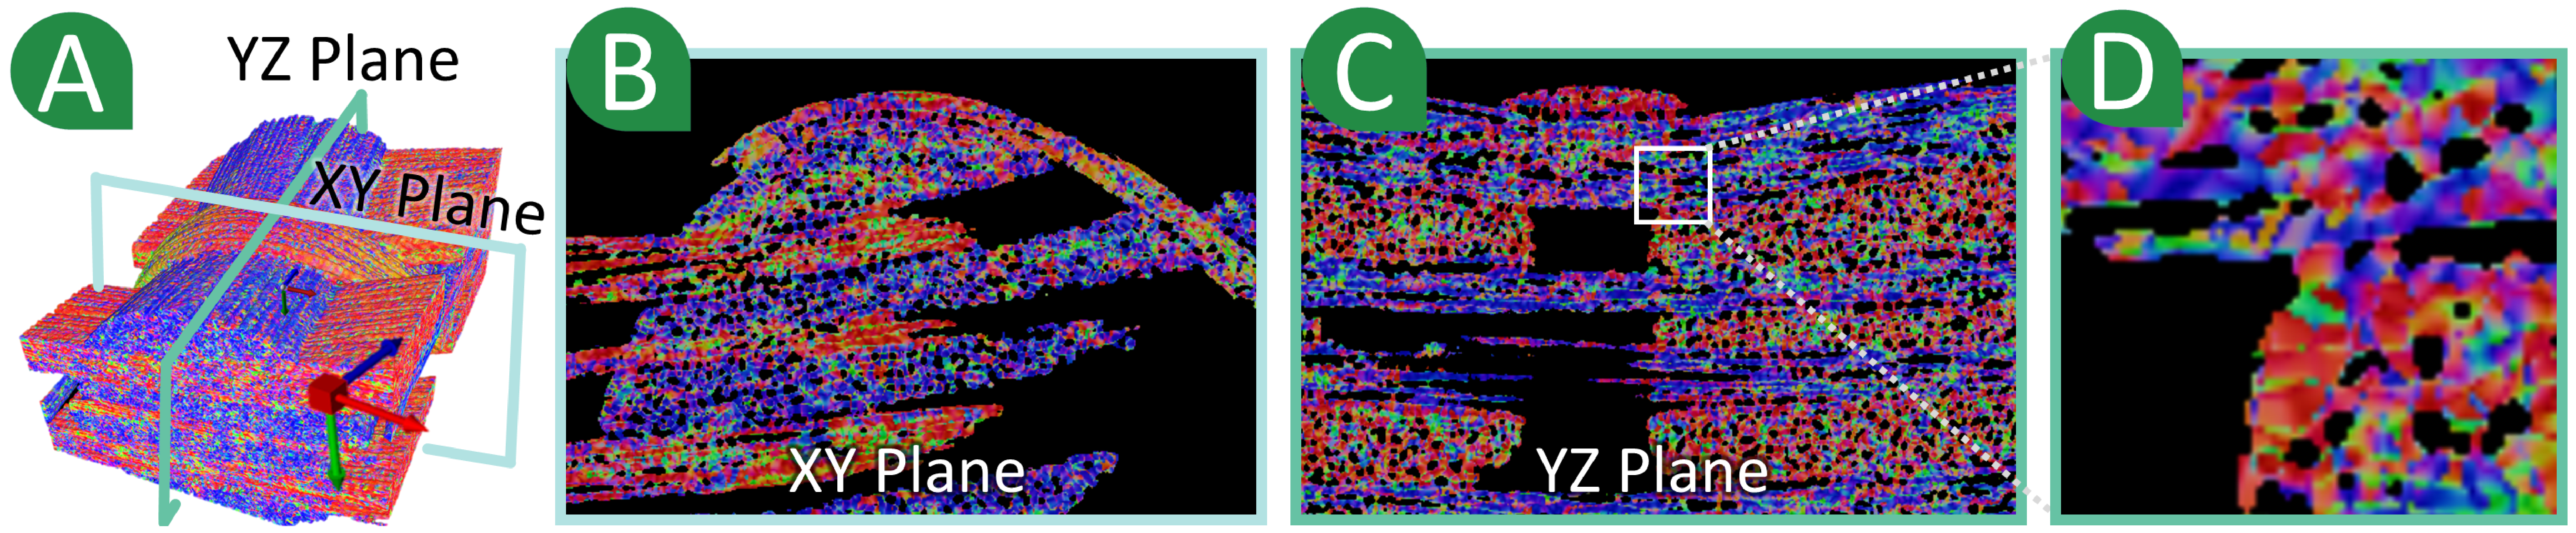
\includegraphics[width=\linewidth]{images_pvis/reliable_hessian.eps}
 \vspace{-1.5em}
\caption{Reliable Hessians. (a) Colored according to Orientation vector mapped to RGB. (b\added{,c}) 2D slice\added{s} along Z\replacedWith{ and (c) along}{-} and X axis. (d) \replacedWith{Magnified}{Zoom in of the white} region marked in \replacedWith{green square}{(c)}.}
\label{fig:reliable_hessian}
\vskip-0.2cm
\end{figure}

Figure~\ref{fig:reliable_hessian}  shows the intermidiate results of local orientation computation.
The unit vector representing the principal direction has been mapped to RGB color space.


 only at locations where $R_{H}$ is greater than the cutoff threshold. The unit vector representing the principal direction has been mapped to RGB color space. Figure~\ref{fig:reliable_hessian}a shows the entire data set. %Regions where the principal direction is parallel to the X axis are red in color, directions parallel to Y are green and those parallel to the Z are blue. 
Figure~\ref{fig:reliable_hessian}b,c show 2D slices along the Z and X axes respectively. Figure~\ref{fig:reliable_hessian}d shows a magnified region of interest. Note, the dark regions within bundles are regions where the $R_H$ is less than the threshold and are unreliable. The bundles are not uniformly colored and the Hessians and the corresponding directions are noisy.

\subsection{\mt Properties}\label{subsec:mt_properties}
\subsection{\mt Generation}\label{subsec:mt_generation}

\section{Fiber Bundle Generation}
\label{subsec:fiber-bundles}
The \mt generated in the previous section represents fragments of fiber bundles. The \mt are clustered in order to extract the final fiber bundles. The clustering process benefits from both the orientation and geometric proximity information inherent in the carbon fiber bundles. Experimentally we found that ``orientation" information was more reliable, while partially overlapping fibers (Figure~\ref{fig:length_distribution}) created problems for ``geometric" proximity based approaches. We also observed that different clustering techniques performed preferably for different measures. 
Instead of creating a heuristic and artificially combining the orientation and geometric proximity measures, we separated the clustering process. 
Specifically, we first cluster based on ``orientation". Each orientation cluster is then further subdivided based on ``geometric" proximity.
The two-step clustering process, helps making the problem more tractable, and the parameters more intuitive to the end users. 
\subsection{Orientation based clustering}
\label {subsec:orientation_clustering}
Before extracting individual fiber bundles, we first separate the \mt into classes based on their major local orientations. To cluster \mt going along similar local directions, we use a spectral embedding technique called Laplacian eigenmaps (originally introduced by Belkin and Niyogi \cite{Belkin01}). An eigenvalue problem is solved to map the manifold embedded in a graph into a lower dimensional space, while preserving the graph structure. 
Let $G$ be the graph, we compute the eigenvalues and eigenvectors for the generalized eigenvector problem $L\textit{\textbf{f}}=\lambda D\textit{\textbf{f}}$,
where $D$ is the diagonal weight matrix and $L$ is the Laplacian matrix. The eigenvector \textbf{${f}_{0}$} corresponding to the eigenvalue 0 is left out and the next $m$, {\textbf{${f}_{1}$} through \textbf{${f}_{m}$}} eigenvectors are used to embed in an $m$-dimensional space (see Sec.~\ref{sec:param_choices} for values of m). 

For our problem, each MetaTract is a node in the graph. We adopt a simple \textit{orientation} based measure to define the weight of the edges. Given a pair of MetaTract, the edge weight between two nodes is defined as the cosine of the maximum angle between the local orientations ($N_P$) of all pairs of start points ($C_P$) between the two MetaTracts. The edge weights give a ``distance matrix" representing the distance between each pair of nodes. Using the Belkin and Niyogi algorithm we ``embed" these nodes in a low dimensional space where the Euclidean distance between nodes, approximates the distance between nodes given by the original ``distance matrix". 
Following this, K-means clustering is employed in the lower dimensional space. Where $K$ is the number of major fiber bundle directions in the woven structure. $K$ is derived from domain knowledge,
for all our test cases, there are two major fiber bundle directions. 
Dimensionality reduction provides us some interesting advantages, by handling the case of curved bundles.
\begin{figure}[htb] 
	\centering  	
	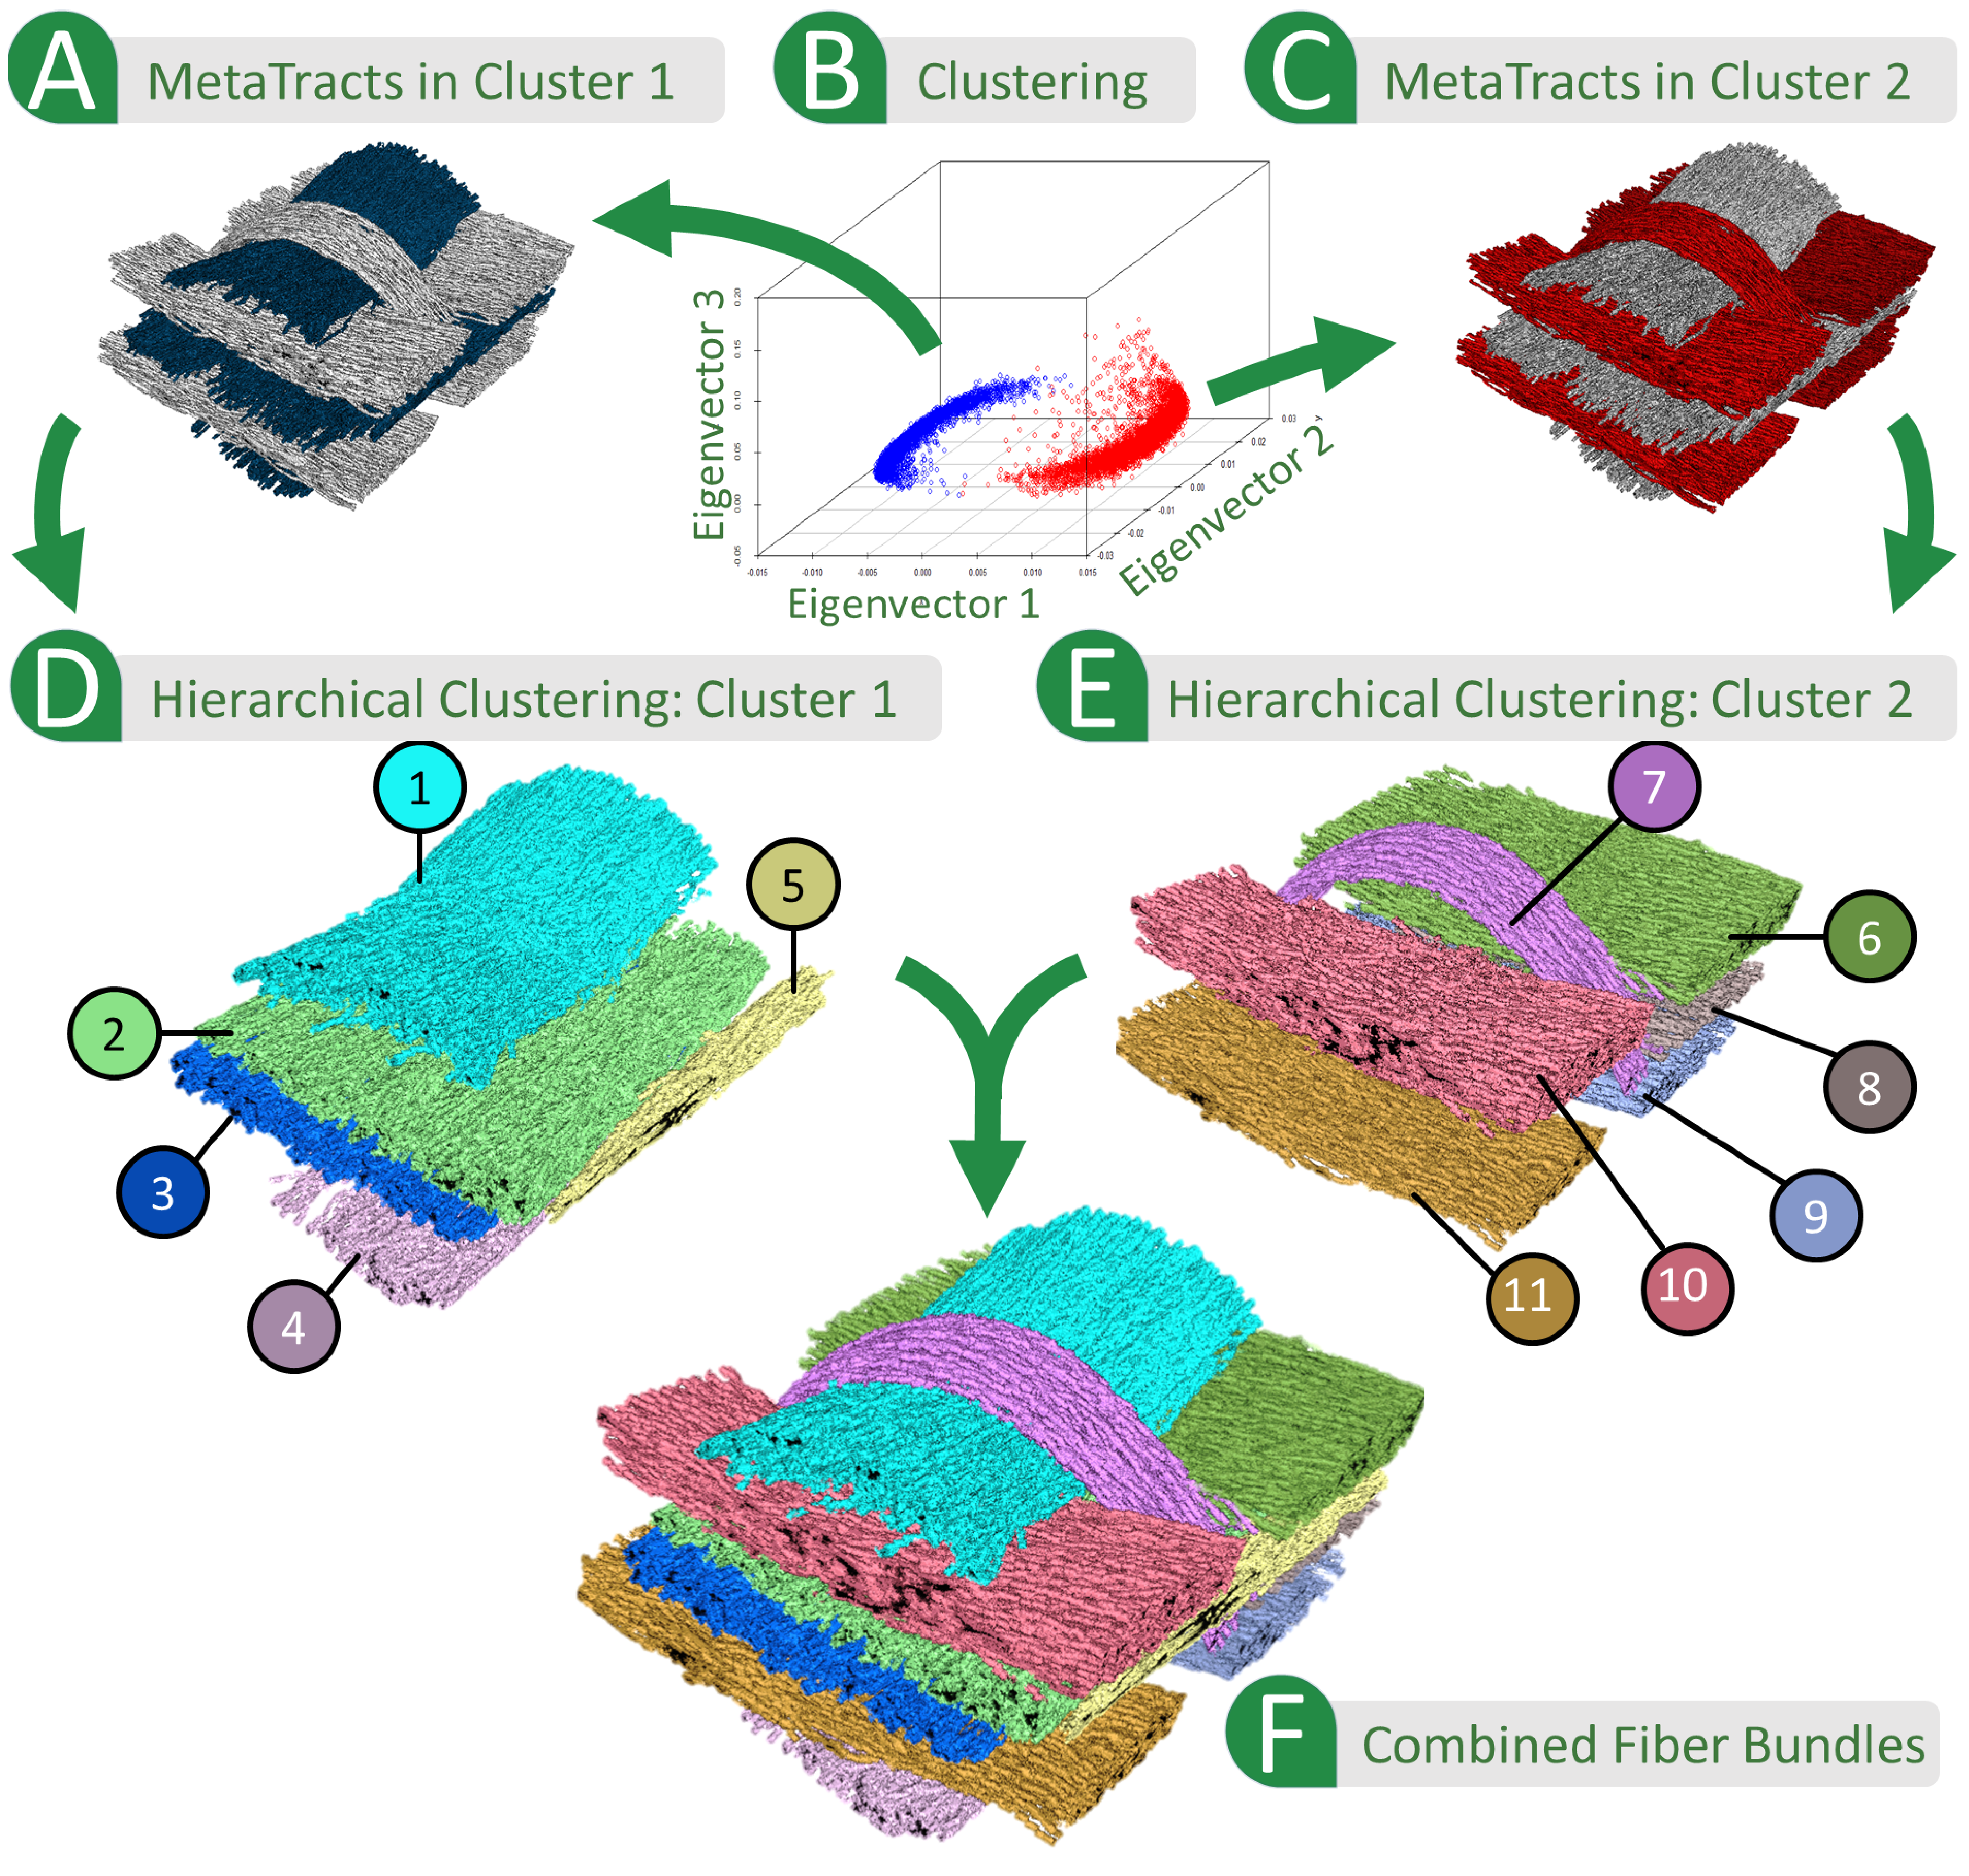
\includegraphics[width=\linewidth]{images/clustering.eps}
	%\includegraphics[width=0.45\textwidth]{imagesMT2014/image_clustering}
	\caption{Clustering Results: Orientation clustering (a,b,c), Distance clustering (d,e).
		 (b) Results of K-means clustering ($K=2$) with \mt (nodes) projected to the top three eigenvectors as major axes. (a) \mt belonging to orientation cluster 1 in blue. (c) \mt belonging to orientation cluster 2 in red, \mt in gray (a,c) show context.
		(d,e) Hierarchical (Distance based) clustering on each orientation cluster. (f) Combined result showing 11 individual extracted clusters. }
	\label{fig:orientation_clustering}
	\vskip-0.2cm
\end{figure} 
Figure~\ref{fig:orientation_clustering}\brac{b} shows the result of the K-means clustering with the nodes (MetaTracts) projected to the top three eigenvectors as the major axes. As expected there is a clear distinction based on fiber bundle orientation. Figure~\ref{fig:orientation_clustering}\brac{a},\brac{c} shows the \mt colored according to orientation clustering results, in blue and red respectively.
Each distinct cluster represents \mt belonging to all fiber bundles, along an individual orientation. 
\subsection{Distance Based Clustering}
\label{subsec:dist_clustering}
To subdivide the oriented clusters into individual fiber bundles, we include further information about the geometric proximity between MetaTracts. We use the directed Hausdorff distance for distance based clustering.
Each MetaTract is represented as a set of points ($C_P$). Formally, the directed Hausdorff distance from point set $P$ to point set $Q$ is defined as 
$H_{dir}(P,Q) = max_{p \in P} min_{q \in Q} d(p,q)$ .
The Hausdorff distance is defined as $H(P,Q) = max(H_{dir}(P,Q),H_{dir}(Q,P))$.
The Hausdorff distance is a metric so $H(P,Q) \le H(P,Q') + H(Q',Q)$ but the directed Hausdorff is not.
%
Unfortunately, the Hausdorff distance does not work well for our application. A single fiber bundle is represented as a set of ``overlapping" MetaTracts. For example  Figure~\ref{fig:length_distribution} shows the length distribution of \mt which express the fiber bundle. Consequently, if a MetaTract $P$ covers only part of the fiber bundle covered by $Q$, then $H_{dir}(P,Q)$ will be very small while $H_{dir}(Q,P)$ will be large.
%
Thus, $H(P,Q)$ will be large, even though $P$ and $Q$ are in the same fiber bundle.
Instead of using the Hausdorff distance, $\max(H_{dir}(P,Q),H_{dir}(Q,P)$, we use $\min(H_{dir}(P,Q),H_{dir}(Q,P))$. If $P$ covers only part of the fiber bundle covered by $Q$, then $\min(H_{dir}(P,Q),H_{dir}(Q,P))$ is very small.
Note that if $P$ and $Q$ overlap but do not cover the same parts of the fiber bundle, then $H_{dir}(P,Q)$ and $H_{dir}(Q,P)$ and $\min(H_{dir}(P,Q),H_{dir}(Q,P))$ will be large.
% 
The directed Hausdorff distance is very sensitive to outliers in the data.
However, because \mt after orientation clustering are constructed using cylinders with similar orientations, they are not plagued by outliers.
To cluster based on MetaTract proximity, we used single linkage hierarchical clustering.
Hierarchical clustering has a single parameter $h$, the desired number of clusters.
Clusters are merged until there are only $h$ clusters left.
Hierarchical clustering is intuitive since it is easy to trace how clusters are formed and merged.
Single linkage clustering finds pairs of objects $p \in P$ and $q \in Q$ where $P \neq Q$ which are closer than other such pairs, and merges the containing clusters $P$ and $Q$.
We found that single linkage hierarchical clustering had two major drawbacks.
\begin{itemize}[nolistsep]
	\item The clustering might produce some ``small" clusters of just a few MetaTracts.
	These \mt are anomalies caused by overlapping fibers and did not represent true fiber bundles.
	\item Second, if two distinct fiber bundles ``ran" parallel for some of their length and then separated, they would sometimes be clustered into a single erroneous bundle.
	This occurs when a short MetaTract which was parallel to both but did not extend into the separation region forms a link between the two fiber bundles. This causes the fiber bundles to be clustered into a single bundle.
\end{itemize}

To address the problem of small clusters, we applied hierarchical clustering and then identified small clusters with few MetaTracts.
We removed the MetaTracts that were in those clusters from the data set and reapplied hierarchical clustering.
To address the problem of short MetaTracts joining different fiber bundles we applied hierarchical clustering and then removed the
shortest tracts (length less than $\eta$ times the median length, set to 0.6) in each bundle. We then reapplied hierarchical clustering.
We repeated both steps until a steady state of clusters was reached and no new small fibers can be removed. The results of hierarchically clustering each orientation cluster ( Figure~\ref{fig:orientation_clustering}\brac{a},\brac{c}) are shown in Figure~\ref{fig:orientation_clustering}\brac{d},\brac{e} respectively.
 
 
After the clustering step, the \mt are separated into well formed fiber bundles. The final result of the clustering process is shown in Figure~\ref{fig:orientation_clustering}\brac{f}. Eleven individual fiber bundles have been separated. Five fiber bundles were extracted from orientation cluster 1 (Z-axis) and six from orientation cluster 2 (X-axis).  
\subsection{Choice of Clustering Techniques}\label{subsec:clus_choice}
\begin{figure}[htb]
	\centering
	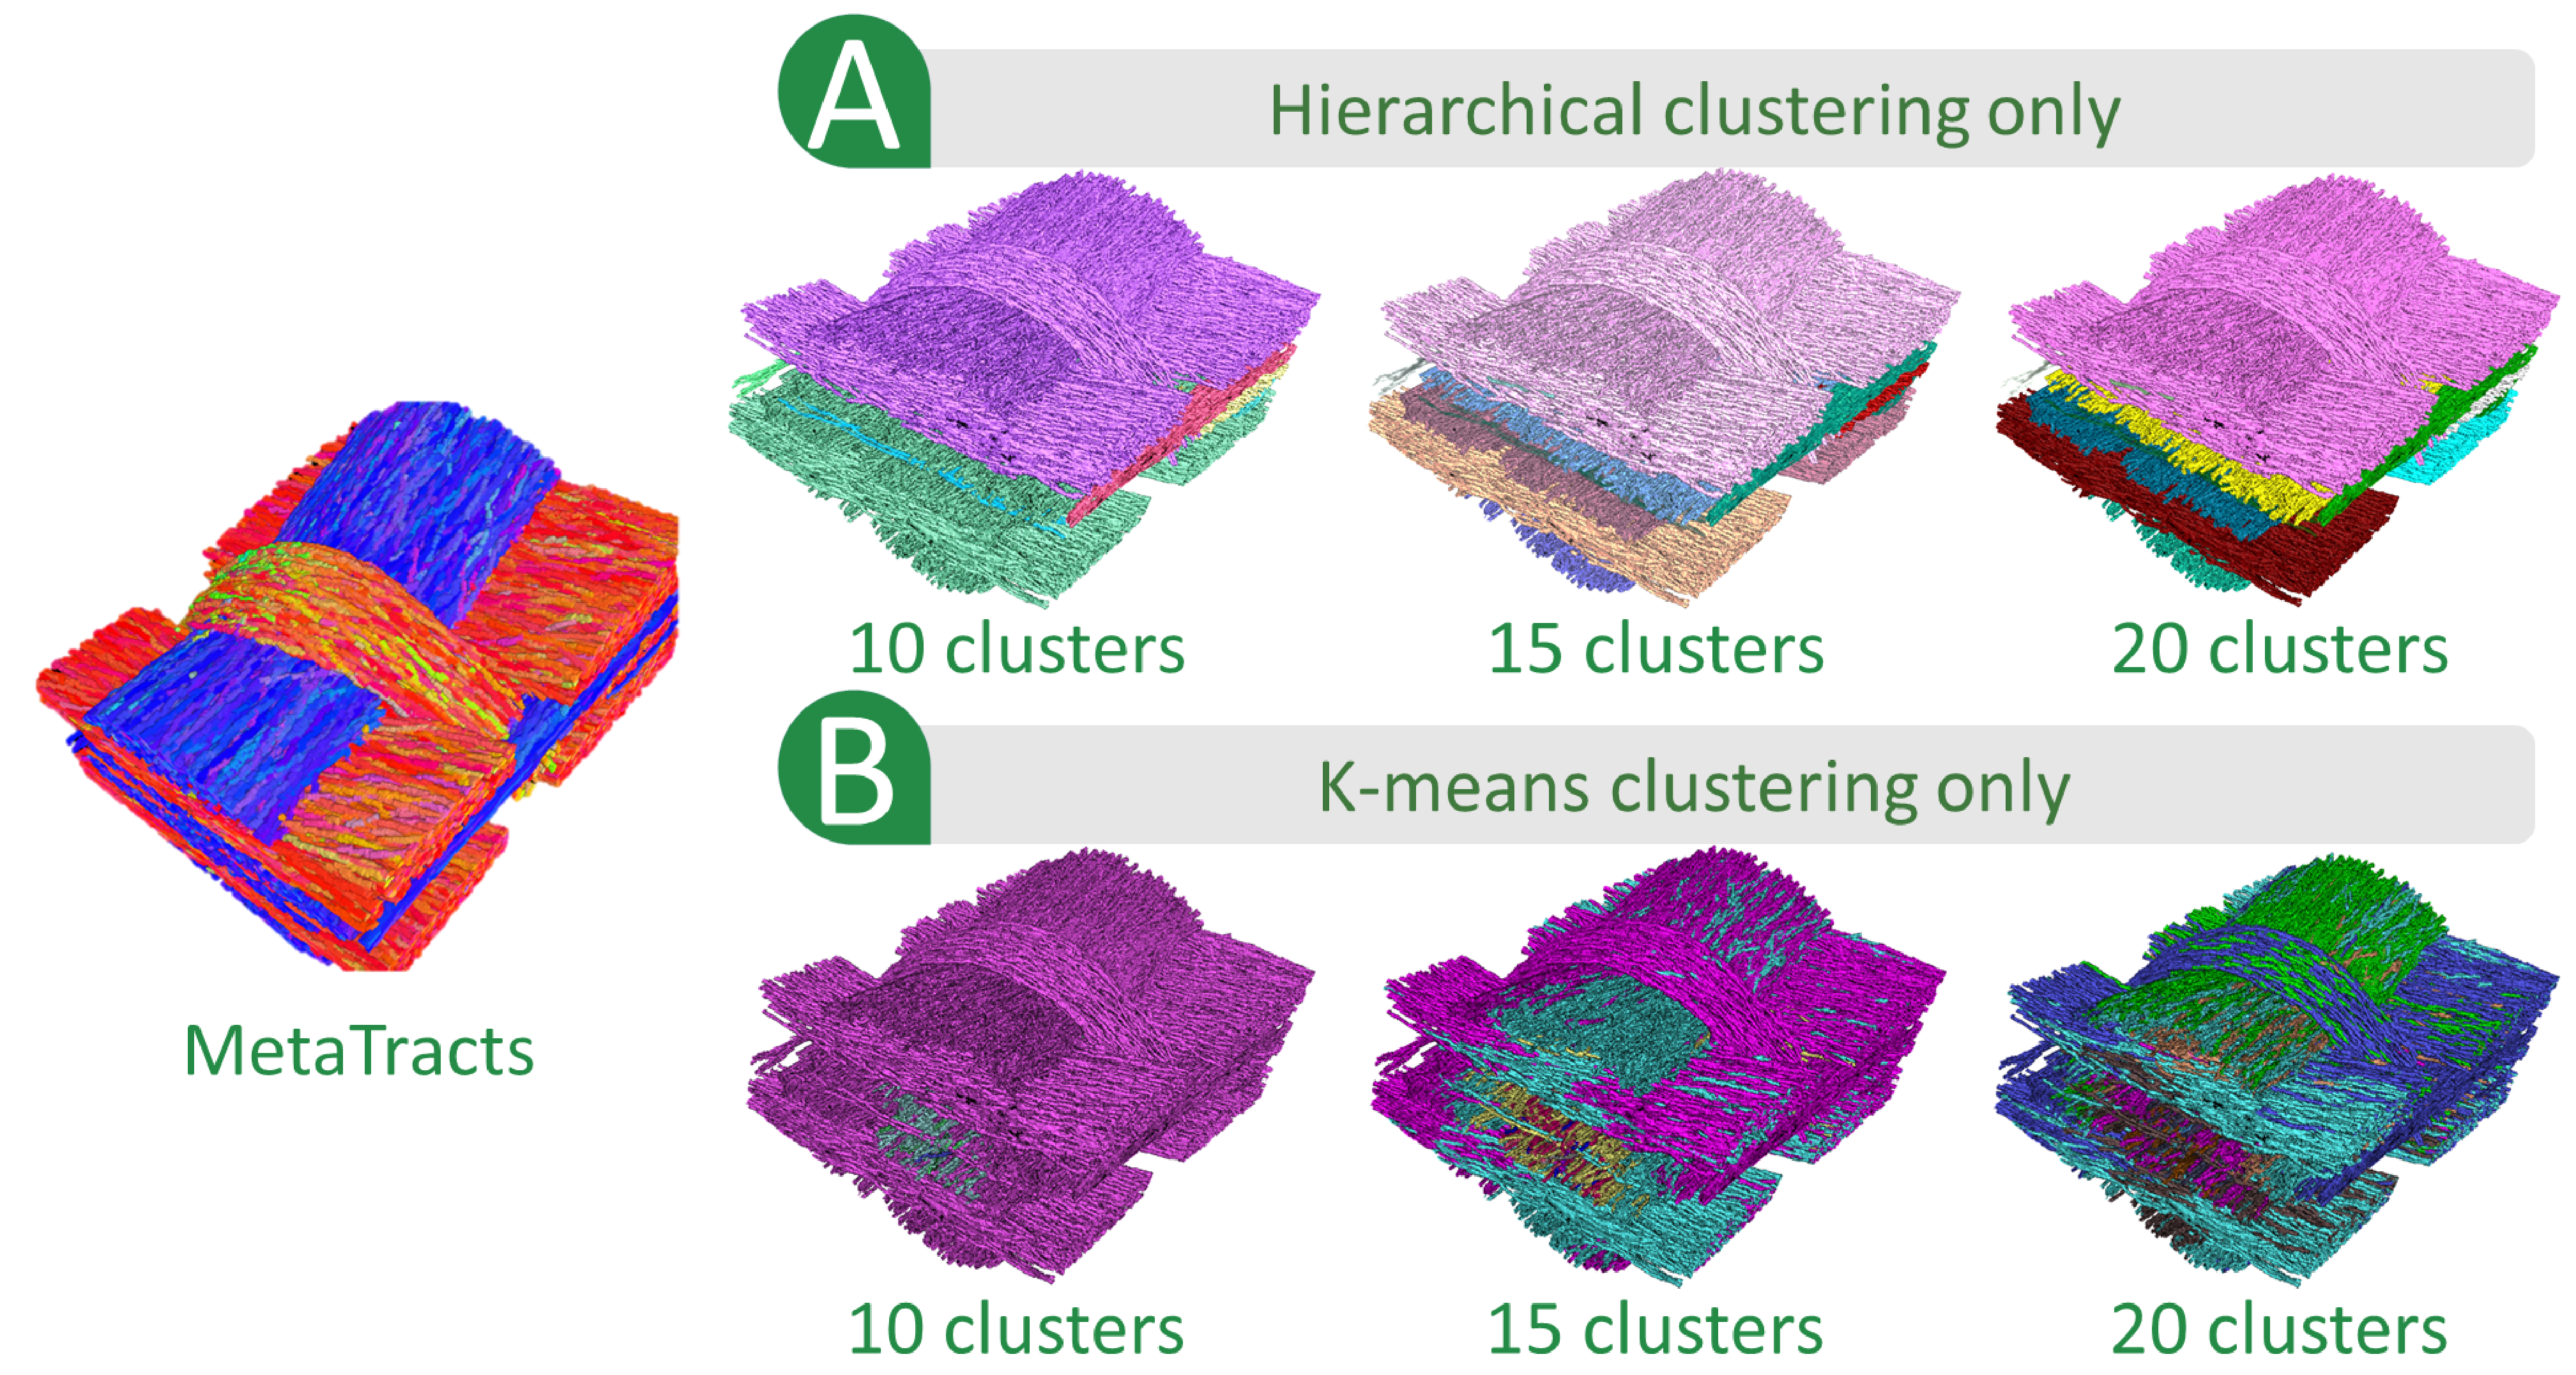
\includegraphics[width=\linewidth]{images/comparison_all.eps}
	\caption{Applying only (a) Hierarchical Clustering and (b) Dimensionality reduction followed by K-means clustering, methods for various numbers of clusters(distance measure is minimal directed Hausdorffs).
		For comparison the results using two-step clustering is in Figure~\ref{fig:orientation_clustering}\brac{f}.}
	\label{fig:comparison}
\end{figure} 
Before settling on the two-step clustering approach, we experimented with using proximity alone, in a single step clustering approach for MetaTracts. We performed two separate tests. First, we used hierarchical clustering to cluster the MetaTracts. Second, we used K-means to cluster the MetaTracts.
Figure~\ref{fig:comparison} shows the results. Figure~\ref{fig:comparison}\brac{a} shows the results of \mt that are hierarchically clustered directly using proximity alone into 10, 15 and finally 20 clusters. 
As discussed in Sec.~\ref{subsec:dist_clustering} single linkage hierarchical clustering in the presence of overlapping \mt tends to create large erroneous clusters and small (low-cardinality) outliers.
When number of clusters (parameter $h$ in hierarchical clustering) is 10, two large incorrect clusters are generated and the rest are outliers. As $h$ increases, some appropriate bundles start to form. But even at $h=20$, fiber bundles incorrectly cluster together. For comparison Figure~\ref{fig:orientation_clustering}\brac{f} shows the two-step clustering result. 


Figure~\ref{fig:comparison}\brac{b} shows the MetaTracts, clustered using K-means clustering by proximity alone, after being embedded in a $m$-dimensional (lower) space. We vary $K$ from 10-20. After the dimensionality reduction, the lower dimensional space does not preserve well the spatial context. As a consequence \mt which are in reality far away are grouped together. Even when k is set to twenty, very few correct fiber bundles are identified.  In comparison, the two-step approach described above is simple, robust and extracts fiber bundles correctly.
\subsection {Sampling \mt}\label{subsec:sampling_mt}
To ensure that the \mt capture the features of all the fiber bundles correctly we uniformly seed the entire volume, which generates a considerably large number of MetaTracts. This increases the time and space requirements of the technique. Especially, orientation clustering which performs eigenvalue and eigenvector computations on large matrices. To ensure that we can handle large datasets and at the same time preserve all features, we start by uniformly seeding the entire volume and generating MetaTracts. We then subsample the \mt and  perform clustering and fiber bundle extraction on these sub-sampled MetaTracts.
The sampling algorithm is given in Algo.~\ref{algo:subsample}. The algorithm  keeps track of a current set of \mt and in each iteration adds the MetaTract furthest from the current set.

Distance between two \mt is measured as the maximum of the minimum distances, between the start points of the cylinders which generate the individual MetaTracts. Computing all pairwise distances is an expensive operation. We bound the distances between a MetaTract to others by maintaining a closest set and compute only when necessary.
\begin{algorithm}[tb]
	$S \leftarrow$ set of all \mt\;
	$n \leftarrow$ number of desired \mt\;
	Pick random MetaTract $M_1 \in S$\;
	$S \leftarrow S -\{M_1\}$\;
	\tcc{Initialization: distances and closest bundle.}
	\ForEach{MetaTract $M \in S$}{
		$M.dist \leftarrow$ distance to $M_1$\;
		$M.closest \leftarrow 1$\;
	}
	\For{$i \leftarrow 2$ \KwTo $n$}{
		Pick the MetaTract $M^* \in S$ with largest $M^*.dist$\;
		$M_i \leftarrow M^*$\;
		Compute the distance from $M_i$ to every $M_j$, $j < i$\;
		$S \leftarrow S - \{M_i\}$\;
		\ForEach{MetaTract $M \in S$}{
			$j \leftarrow M.closest$\;
			\If{($d(M_j,M_i) < 2*M.dist$)}{
				Compute $dist(M,M_i)$\;
				\If{$(dist(M,M_i) < M.dist)$}{
					$M.dist \leftarrow dist(M, M_i)$\;
					$M.closest \leftarrow i$\;
				}
			}
		}
	}
	\caption{Algorithm to subsample MetaTracts.}
	\label{algo:subsample}
\end{algorithm}
With the sampling step the user can decide the ``resolution" of \mt by setting the parameter $n$ based on their requirements and computational constraints (see Sec.\ref{sec:param_choices}).
\section{Visualization of \mt}
\label{sec:vis}
The output of the clustering step, can be used to visualize the geometric structure of the fiber bundles and answer the general queries itemized in Sec.~\ref{sec:intro}. Apart from the direct \mt visualization, we added three additional extensions which were requested by the domain specialists as highly important and useful. Specifically, 
\begin{itemize}[noitemsep,nolistsep]
	\item The first extension is to voxelize the original volume according to the clusters each voxel is associated with.
	\item The second extension is to extract surfaces (triangle meshes) associated with each fiber bundle. 
	\item Finally, we added an interactive tool which allows complete visual analysis of the fiber bundles. 
\end{itemize}
\subsection{Voxelization and surface extraction}\label{subsec:voxel_surf_extraction}
To voxelize the entire volume based on the clustering results of the MetaTracts, we take the following ``voting" approach.
We compute a neighborhood around each voxel. We then create a histogram by  enumerating the number of voxels of each class (cluster) in this neighborhood. The voxel is then assigned to the class with the maximum number of elements in the neighborhood. 
Surface extraction is often a crucial requirement for post processing of the data. While Marching Cubes\cite{Lorensen1987} remains the most popular technique, other methods specific to ICT data such as MergeSharp~\cite{Bhattacharya2013} which focuses on extracting sharp edges and corners are also used.  
We extract the corresponding surfaces from voxel data by binarizing the volume per cluster and extracting the isosurface associated with the largest connected component in the input binary volume. 
\begin{figure}[htb]
	\centering
	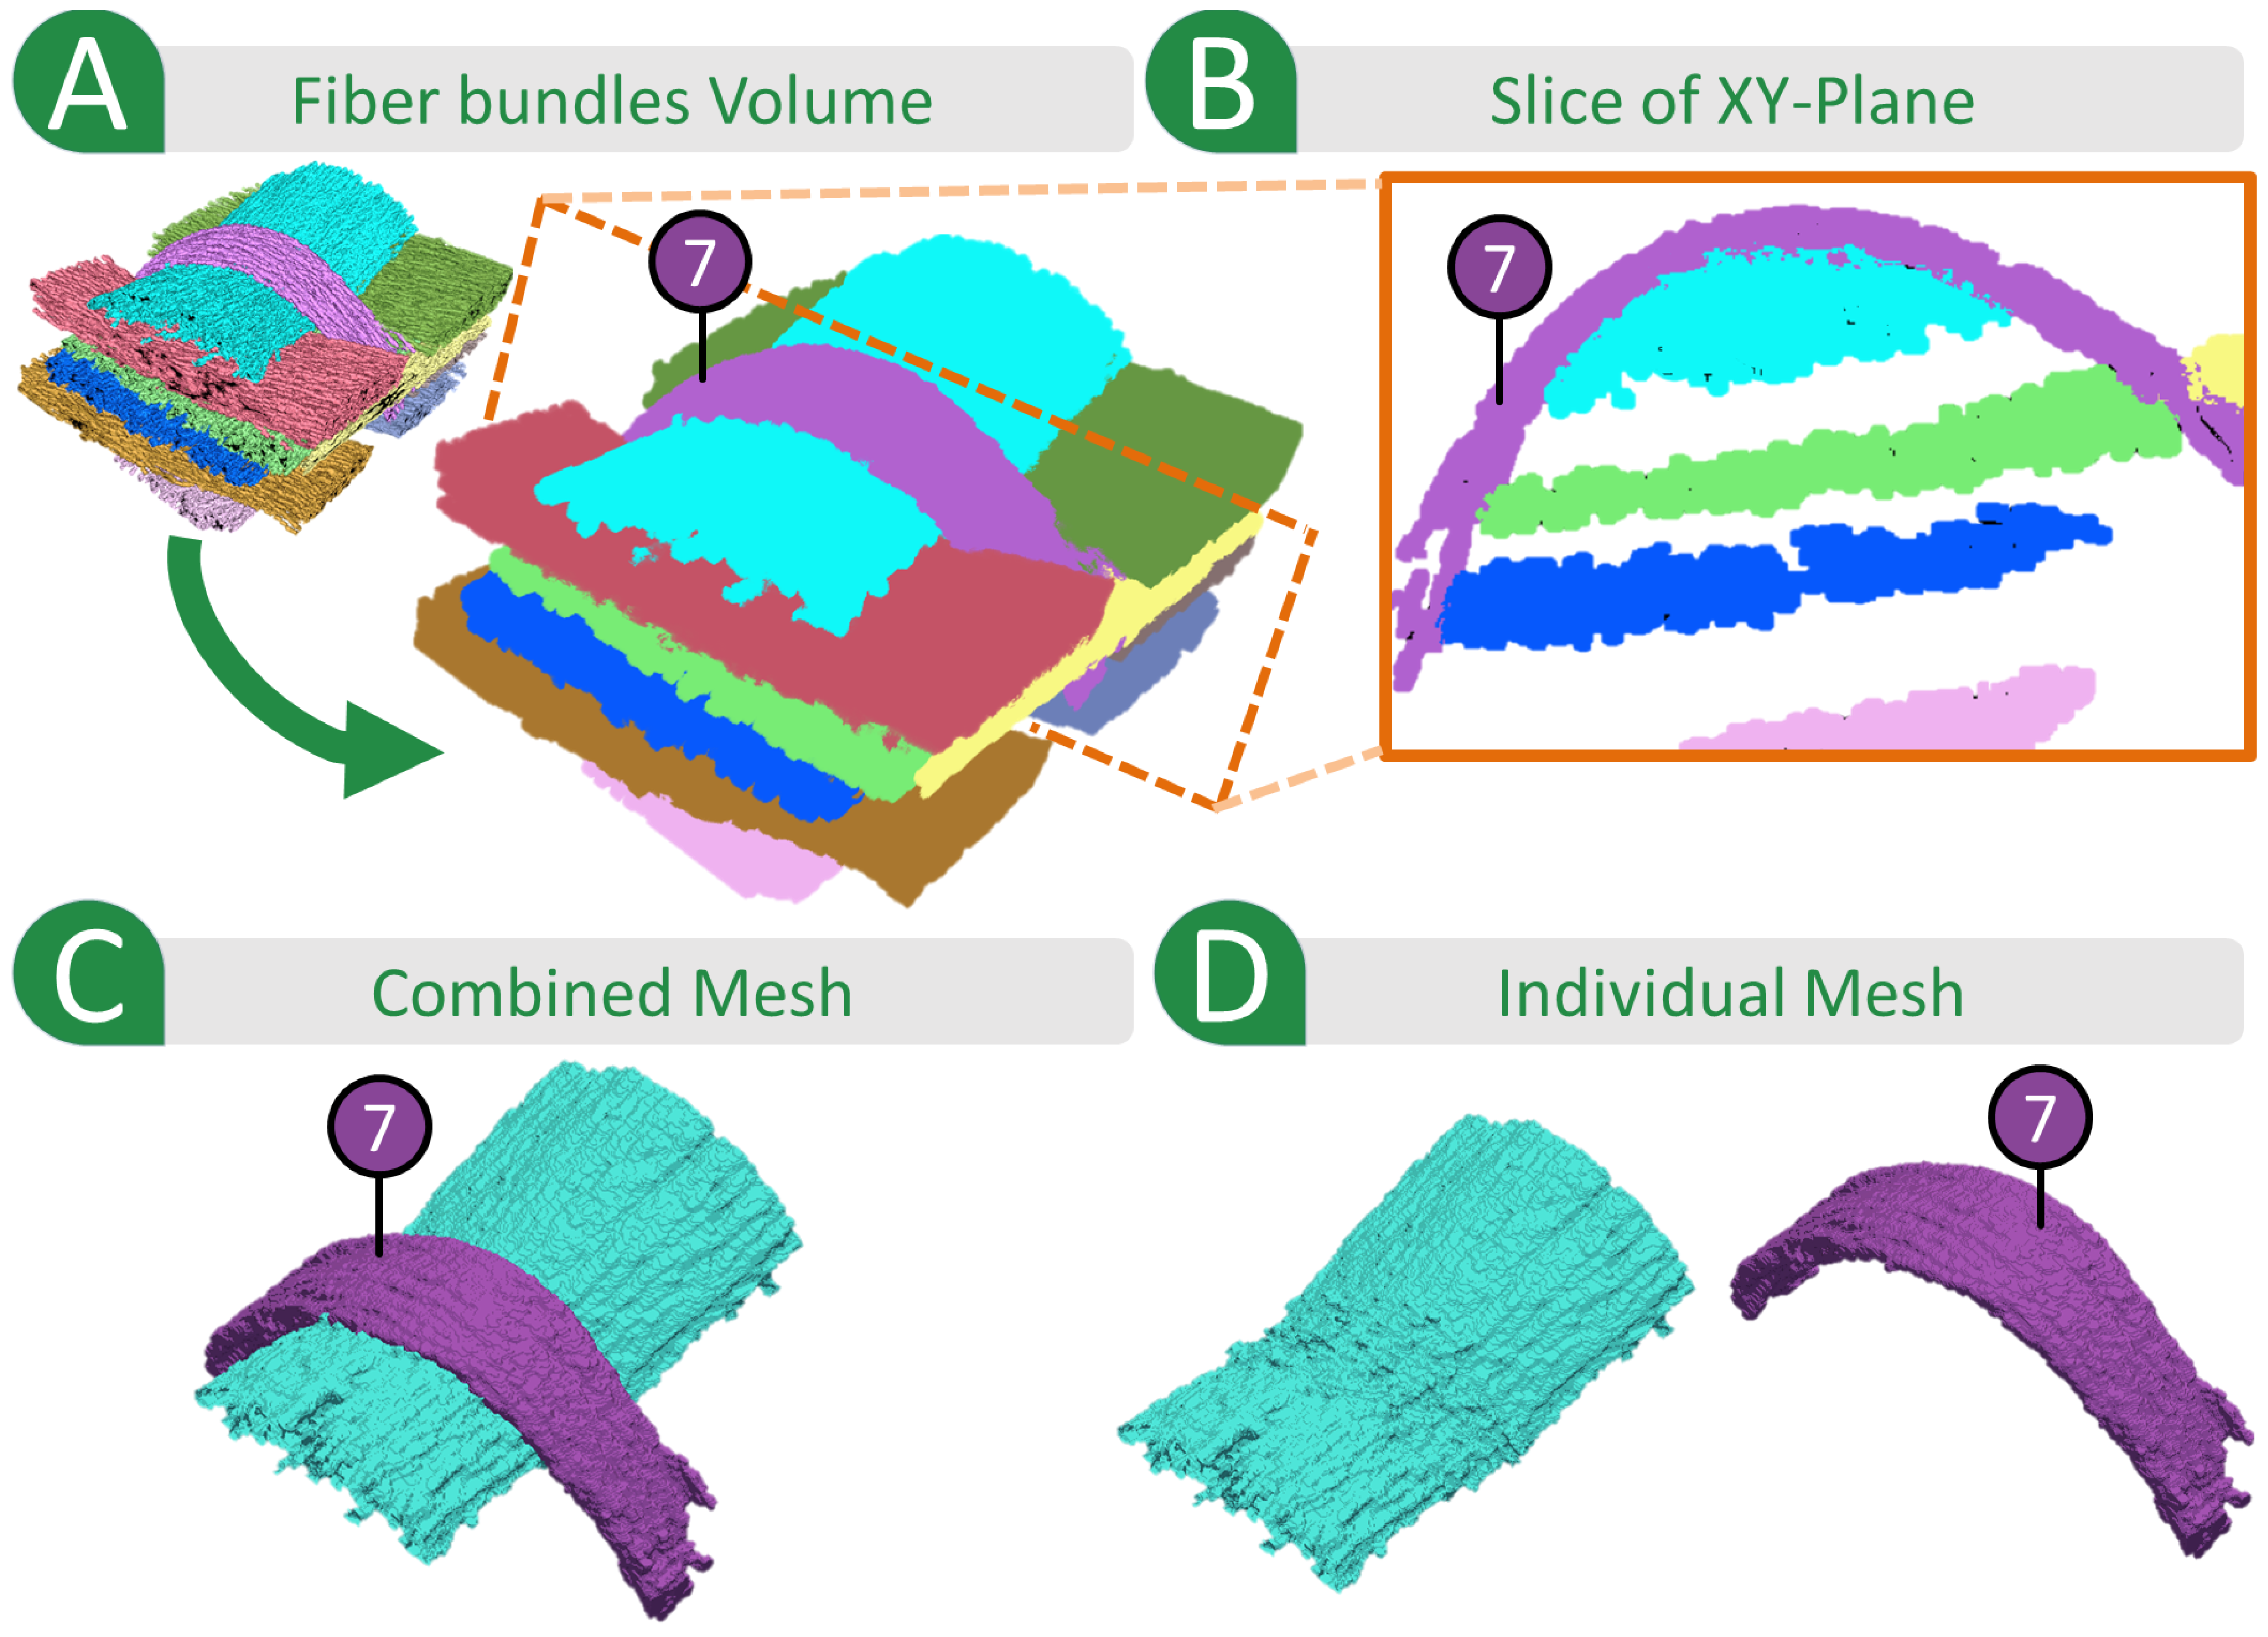
\includegraphics[width=\linewidth]{images/figure8.eps} 
	\caption{Voxelization and surface extraction. (a) Voxelization of data set 1, the inset shows the \mt after clustering. (b) a single slice along the XY-Plane (c) Two of the extracted meshes together (d) The meshes rendered separately.}
	\label{fig:crop-16-decomp}
\end{figure} 
Figure~\ref{fig:crop-16-decomp}\brac{a} and~\ref{fig:prepreg}\brac{d} show the result of voxelization. Figure~\ref{fig:crop-16-decomp}\brac{b} shows a single slice of the volume along the XY-plane. Figure~\ref{fig:crop-16-decomp}\brac{c},\brac{d} shows examples of extracted meshes.



\section{Experimental Results}
\section{Parameter Choices}\label{sec:param_choices}
The critical parameters for \mt are $K$ and $h$, where parameter $K$ is used by the K-means during orientation clustering while parameter $h$ which is used by the hierarchical clustering.
K denotes the number of major fiber bundle directions. This is known a priori or can be estimated by considering the weaving pattern. 
\begin{figure}[tb]
	\centering
	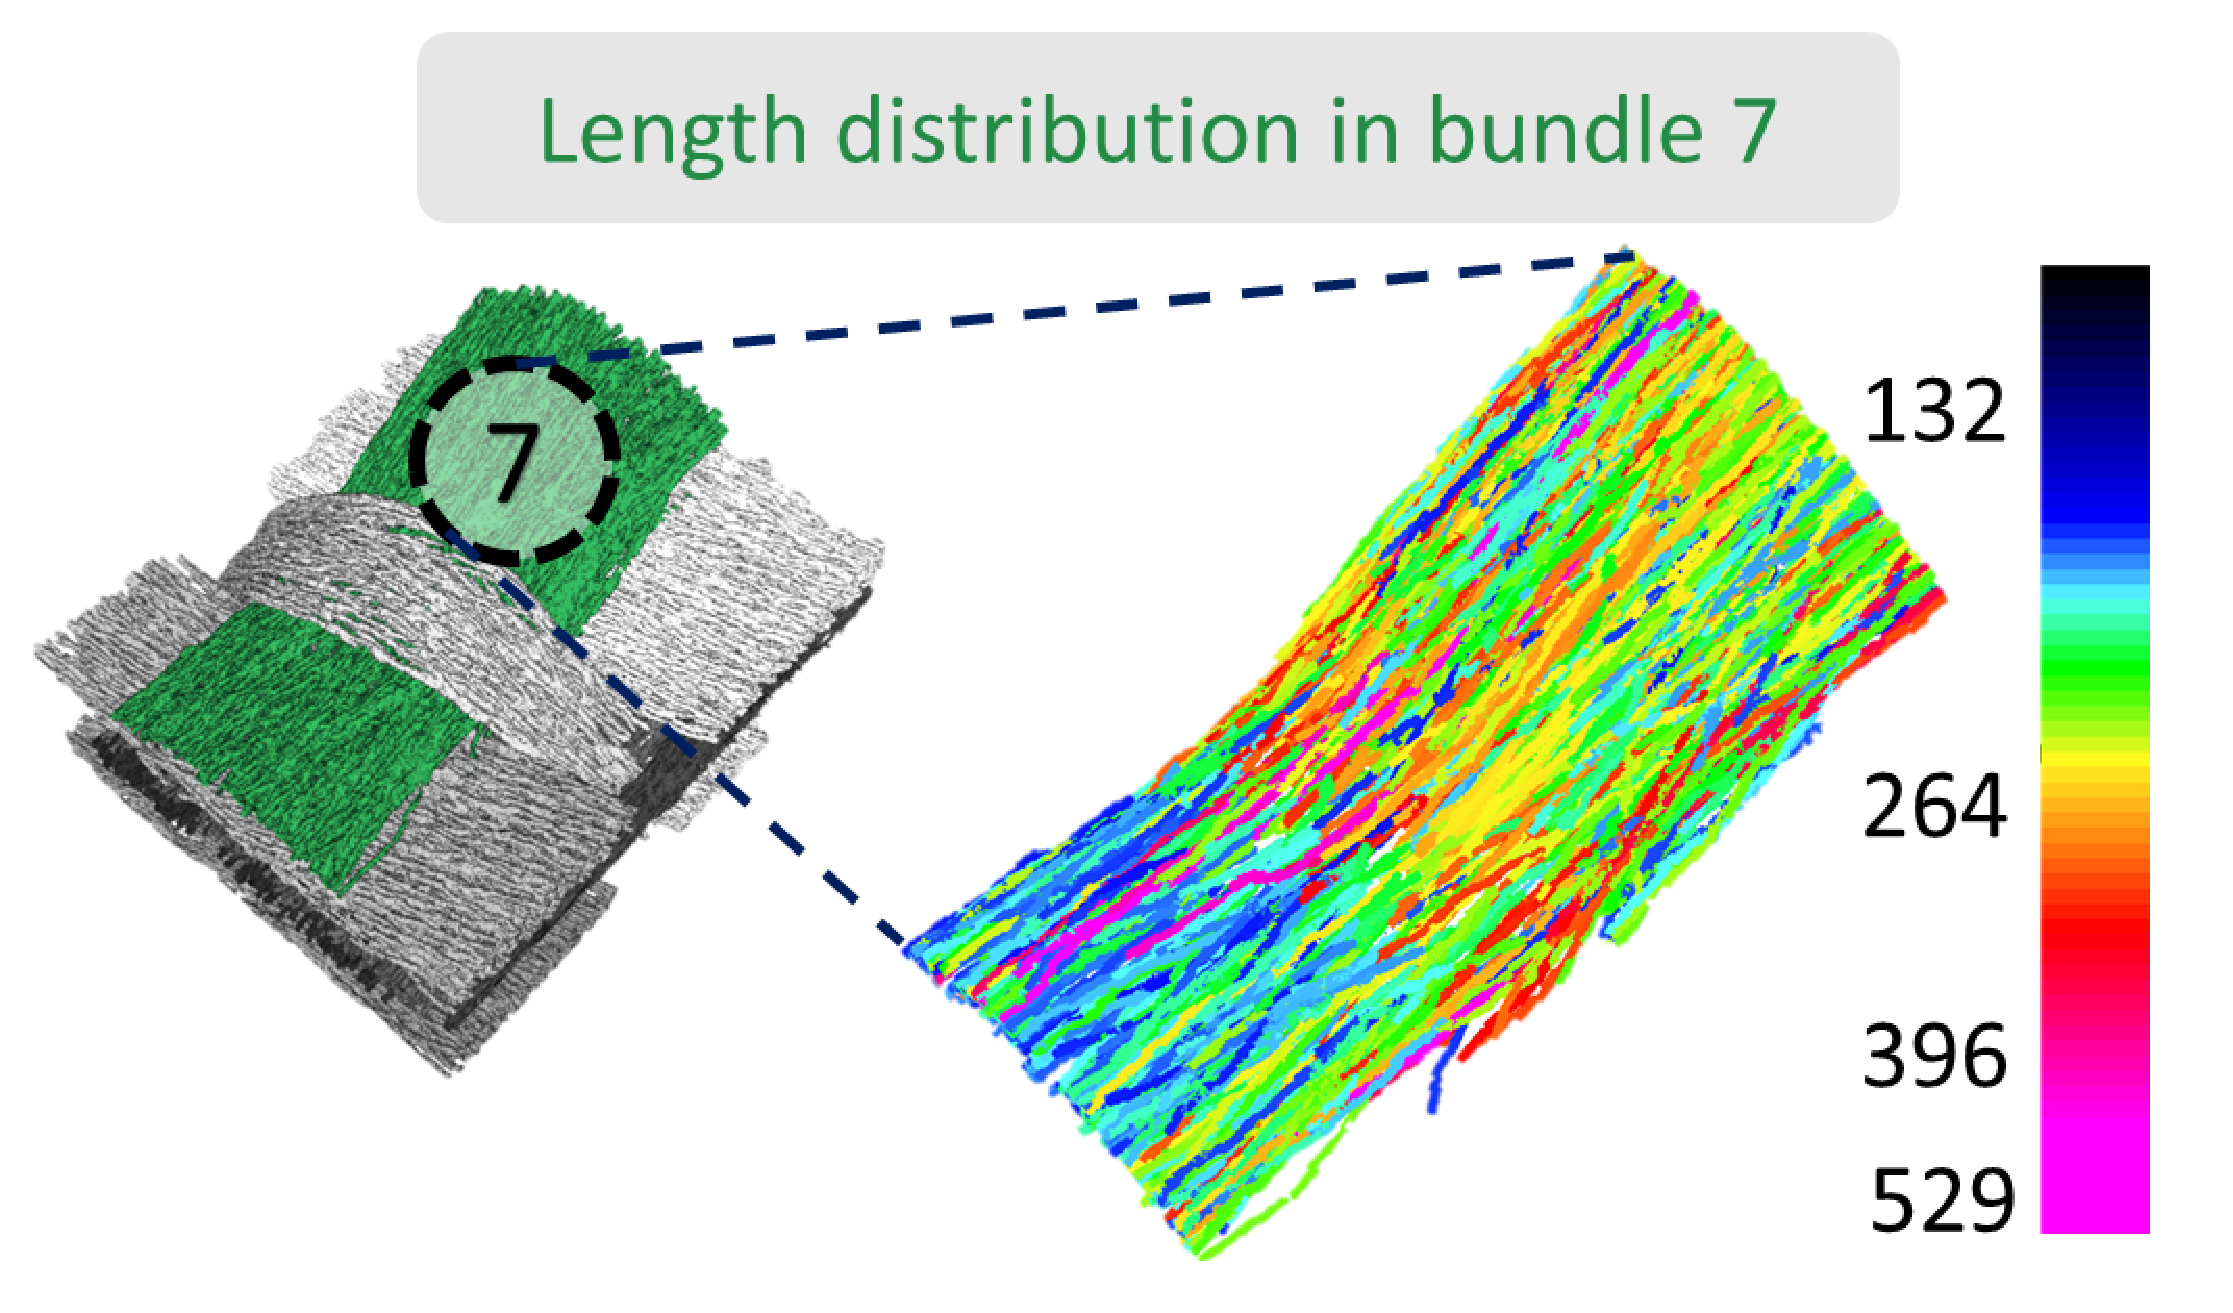
\includegraphics[width=0.8\linewidth]{images/lengthDistribution.eps}
	\caption{(a) Length distribution of individual \mt for a particular bundle (unit for length is grid cube edge length:  $2\mu m$).}
	\label{fig:length_distribution}
\end{figure}
\begin{figure}[tb]
	\centering
	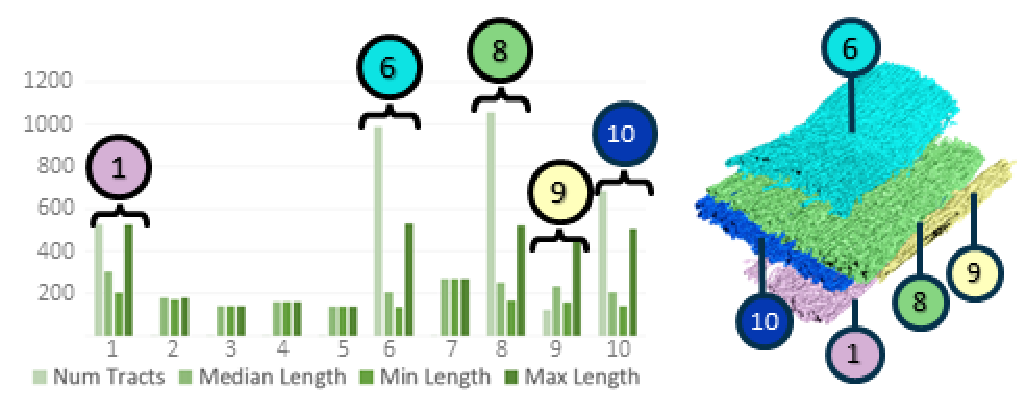
\includegraphics[width=\linewidth,  trim = 0mm 0mm 0mm 00mm, clip]{images/figure9_AMA.eps}
	\caption{Number of \mt and median, minimum and maximum length of an individual MetaTracts in the orientation cluster Figure~\ref{fig:orientation_clustering}\brac{d} when clustered into 10 clusters. The unit for the MetaTracts length is the grid cube length. The labeled clusters 2, 3, 4, 5 and 7 have a cardinality less than 10 and are removed. }
	\label{fig:len_dist_crop16} 
\end{figure}
Figure~\ref{fig:len_dist_crop16} shows the number of \mt in each cluster when the orientation cluster 1 (Figure ~\ref{fig:orientation_clustering}\brac{a}) is hierarchically clustered into ($h$) 10 clusters. It also shows the minimum, maximum and median length of the MetaTracts in each of the resulting clusters. The ground truth was five separate fiber bundles. We observe that the major fiber bundles remain well separated in accordance with our ground truth and the small clusters (clusters 2, 3, 4, 5 and 7) have very few elements and can be easily discarded. Thus we see that our framework is robust to the choice of parameter $h$ for hierarchical clustering. This is an appealing trait of the proximity based hierarchical clustering, thus providing good results even when exact $h$ might be unknown. The robustness to parameter variation also reinforces our two-step approach to clustering. 


The following parameters were fixed for all the tests. We set the reliable Hessian threshold $R_{H}$ to be 0.3. A $R_{H}$ of 0.0 would mean all points have reliable local orientation which would cause spurious MetaTracts detection. A very high $ R_{H}$ would lead to a decline in number of MetaTracts produced. Coefficients $\alpha$ and $\beta$ in $R_{H}$ are as explained in Frangi et al.~\cite{Frangi1998} and set to 0.5. The length and the radius parameters for the cylinders of MetaTracts decide how coarse our approximation of the fiber bundles are. These are dependent on the underlying fiber characteristic and the weaving pattern. Larger cylinders will handle noisy local orientation better as it inspects a larger number of candidate points to extend the fiber. We used 10 and 2 for length and radius (measured in grid voxel size), respectively for all tests.  
A simpler geometry (e.g., D2) was experimentally found to handle larger cylinders better. $\eta$ in Sec.~\ref{subsec:dist_clustering} decides how quickly the hierarchical clustering converges, experimentally values 0.3 to 0.6 removed $1.2\% - 5\%$ of fibers (total number of fibers $\sim$10000) and gave similar results. We set $n$ the number of sampled \mt to 10.000 for all our test cases. Parameter $n$ intuitively acts as ``resolution" for the MetaTracts. Large $n$ captures the features better and generates smoother fiber bundles. 

$\alpha$ and $\beta$ in equation~\ref{eqn:algo_1} decide how quickly the value of the factor decays; we have used integer values between [7-10] and half the length of an individual cylinder respectively. Our number of fiber bundle directions is limited. Thus even for small $m$ (cardinality of lower dimension in orientation clustering), the distinction between the orientation clusters is preserved quite well. We compared $m=3,...,7$ experimentally without any change in results. 
\section{Limitations}\label{sec:limitations}
A key assumption of the method is ``connectivity'' (Sec.~\ref{sec:char_data}).
If the ``connectivity'' criteria is not fulfilled due to noise in the image, then the generated MetaTracts will be inaccurate. 
The clustering process also assumes that the fiber bundles have a minimum width.
\section{Conclusions and Future Work}\label{subsec:conclusions}
In this paper, we introduce a framework to extract and visualize fiber bundles in composite materials. We show that our framework works at comparatively low resolution and with dense fiber arrangements (when extracting single fibers might not be possible). It handles complex fiber patterns such as ``cross overs'' and ``braiding''.
In addition, we demonstrated a tool to interactively investigate and analyze voxelized fiber bundles generated with the MetaTracts approach.

In future, we plan to increase the precision of the extractions, include uncertainty based visualization to better portray the surface of separations and speed up extraction times.

%% if specified like this the section will be committed in review mode
\acknowledgments{
The authors wish to thank A, B, C. This work was supported in part by
a grant from XYZ.}

\bibliographystyle{abbrv}
%%use following if all content of bibtex file should be shown
%\nocite{*}
\bibliography{metaTracts}
\end{document}

